\article{Shimura 簇：模解释与典范模型的构造技术}{Variétés de Shimura : interprétation modulaire, et techniques de construction de modèles canoniques}{Pierre Deligne}{2}{247--289}
\paragraph*{篇内目录。} 引言（原247页）；回顾、术语和记号（250）；1. Hermitian 对称域（251）：1.1 Hodge 结构的模空间（251），1.2 分类（257），1.3 辛嵌入（259）；2. Shimura 簇（262）：2.0 预备知识（262），2.1 Shimura 簇（265），2.2 典范模型（268），2.3 典范模型的构造（270），2.4 互反律：预备知识（274），2.5 应用：一个典范扩张（280），2.6 典范模型的互反律（284），2.7 归结到导出群及存在定理（285）；参考文献（289）。

\origsection{}{引言（Introduction）}
本文接续 [5] 的讨论，并使用其中第4、5节的主要结果。第一部分说明定义 Shimura 簇（Shimura varieties）时，系统 $(G,X)$（2.1.1）所须满足的公理从何而来。我们证明，大致而言，它们对应于下列类型的 Hodge 结构（Hodge structures）的模空间（moduli spaces）$X^+$。\footnote{原文 AMS（MOS）学科分类（1970）：主要10D20、14G99；次要20G15、20G30。}

(a) 在固定向量空间 $V$ 上，要求某些张量 $t_1,\ldots,t_n$ 为 $(0,0)$ 型的所有 Hodge 结构组成的空间，$X^+$ 是其一个连通分支。代数群 $G$ 是固定各 $t_i$ 的 $\GL(V)$ 子群，而 $X=G(\R)\cdot X^+$ 是其轨道。

(b) 由 $X^+$ 参数化的 Hodge 结构族满足代数几何中自然出现的 Hodge 结构族所具有的条件：$X^+$ 有适当且唯一确定的复结构，使该族成为可极化 Hodge 结构变分（polarizable variation of Hodge structure）。

空间 $X^+$ 自动为 Hermitian 对称域（Hermitian symmetric domain），即曲率小于零的 Hermitian 对称空间。所有 Hermitian 对称域都可如此描述为 Hodge 结构的模空间（1.1.17），我认为这种描述很有用。例如，$D$ 嵌入其对偶 $\check D$（一个旗簇（flag variety）），对应于将 Hodge 结构映到相应 Hodge 滤过（Hodge filtration）的映射。“第三类 Siegel 域”的描述可解释为：在某些假设下，将权滤过（weight filtration）叠加在 Hodge 结构上得到混合 Hodge 结构（mixed Hodge structure），从而有从 $D$ 到混合 Hodge 结构模空间的映射，参见 [1，III，4.1]。本文既不再提及也不使用这一点。

上述观点与将某些 Shimura 簇描述为阿贝尔簇（abelian varieties）模空间的观点，通过以下对应联系起来：给出阿贝尔簇，等价于给出无挠的、类型为 $\{(-1,0),(0,-1)\}$ 的可极化 $\Z$ Hodge 结构，范畴等价由 $A\mapsto H_1(A,\Z)$ 给出。改取对偶 $A\mapsto H^1(A,\Z)$ 后，可用 $\{(1,0),(0,1)\}$ 代替。给阿贝尔簇赋予极化，等价于给其 $H_1$ 赋予极化。这一对应也适用于带参数的情形：在光滑复簇 $S$ 上给出极化阿贝尔概形（polarized abelian scheme），等价于在 $S^{\mathrm{an}}$ 上给出类型为 $\{(-1,0),(0,-1)\}$ 的极化 Hodge 结构变分。由 $S^{\mathrm{an}}$ 参数化的阿贝尔簇解析族自动为代数的，见 [3]。要解释更复杂类型的 Hodge 结构，人们希望以适当“动机”（motives）代替阿贝尔簇，目前这还只是梦想。

1.2利用上述框架，以 Dynkin 图及其特殊顶点描述 Hermitian 对称域的分类。1.3则对某类到 Siegel 半空间的嵌入作出分类，所得结果与 Satake [11] 相对应。应用 Weyl 酉技巧（unitary trick，见 [7]），分类归结为查阅基本权按简单根展开的系数表；所需表格可见 Bourbaki [4]。

关于 Hodge 结构变分及其在代数几何中的出现，读者可参阅 [6]（我们的符号约定与之不同）；[6] 陈述的某些事实证明于 [7]。

2.1、2.2用阿代尔语言定义 Shimura 簇 ${}_KM_{\C}(G,X)$（[5] 中记为 ${}_KM_{\C}(G,h)$，$h\in X$ 任意）、其投射极限 $M_{\C}(G,X)$ 及典范模型（canonical model）。具体定义见正文；这里只说，典范模型是在对偶域（reflex field；原文 corps dual，2.2.1）$E(G,X)$ 上的概形 $M(G,X)$，配有同构
\[
 M(G,X)\otimes_{E(G,X)}\C\xrightarrow{\sim}M_{\C}(G,X),
\]
且这种定义域下降满足适当性质：$G(A^f)$ 等变性及特殊点（special points，2.2.4）的 Galois 性质。还定义弱典范模型（weakly canonical model）：同一定义中，将 $E(G,X)$ 换成包含于 $\C$ 的某个有限扩张 $E$。它在构造典范模型时起技术作用。2.1、2.2的定义与 [5] 在表述上的差异，来自符号约定的不同，如右作用与左作用、整体类域论互反律的选择。

启发性描述见 [5] 引言；从阿代尔语言过渡到经典语言的简短例子见 [5，1.6--1.11、3.14--3.16、4.11--4.16]。

[5] 将 Shimura 构造典范模型的方法系统化。本文第二部分改进其结果。2.6在假定 $M_{\C}(G,X)$ 存在 $E$ 上弱典范模型的前提下，确定 $\Gal(\overline\Q/E)$ 在其几何连通分支集上的作用，不再像 [5] 那样假设 $G^{\mathrm{der}}$ 单连通。关键在于2.4构造的下述态射：设 $G$ 为 $\Q$ 上连通约化群，$\rho:\widetilde G\to G$ 为导出群 $G^{\mathrm{der}}$ 的万有覆盖，$M$ 为定义于数域 $E$ 的 $\Gm\to G$ 同态共轭类。构造从 $E$ 的伊代尔类群（idele class group）到阿贝尔商 $G(A)/\rho\widetilde G(A)G(\Q)$ 的同态 $q_M$。它对 $(G,M)$ 函子化，且 $F/E$ 扩张时，下图交换：
\[
 \begin{tikzcd}
 C(F)\arrow[d,"N_{F/E}"']\arrow[dr]&\\
 C(E)\arrow[r]&G(A)/\rho\widetilde G(A)G(\Q).
 \end{tikzcd}
\]
若 $\widetilde G$ 没有使 $G'(\R)$ 紧的 $\Q$ 因子 $G'$，由强逼近定理得到
\[
 \pi_0(G(A)/\rho\widetilde G(A)G(\Q))=\pi_0(G(A)/G(\Q)).
\]
由整体类域论，$\pi_0C(E)$ 为阿贝尔化 Galois 群 $\Gal(\overline\Q/E)^{\mathrm{ab}}$，$q_M$ 给出它在此连通分支集上的作用。

第二个新想法其实是回到 Shimura 的观点。由2.6可从弱典范模型的中性分支 $M_{\overline\Q}^0(G,X^+)$，连同稳定它的 $G(A^f)\times\Gal(\overline\Q/E)$ 子群 $H$ 的半线性作用，重建模型 $M_E(G,X)$。该几何连通分支依赖于 $X$ 的连通分支 $X^+$。设 $Z$ 为中心，$G^{\mathrm{ad}}$ 为伴随群，$G^{\mathrm{ad}}(\R)^+$ 为实点的拓扑中性分支，$G^{\mathrm{ad}}(\Q)^+=G^{\mathrm{ad}}(\Q)\cap G^{\mathrm{ad}}(\R)^+$。$Z(\Q)$ 在 $G(A^f)$ 中的闭包 $Z(\Q)^-$ 平凡作用，故 $H$ 的作用经 $H/Z(\Q)^-$ 分解。实际上可让一个稍大的群作用，它是 $\Gal(\overline\Q/E)$ 关于 $G^{\mathrm{ad}}(\Q)^+$ 的某个完备化的扩张，完备化的拓扑由 $G^{\mathrm{der}}(\Q)$ 同余子群的像给出。

此扩张在唯一同构的意义下唯一确定，只依赖 $G^{\mathrm{ad}},G^{\mathrm{der}}$ 及 $X^+$ 在 $G^{\mathrm{ad}}$ 中的像 $X^{+\mathrm{ad}}$（2.5），记为 $\mathcal E_E(G^{\mathrm{ad}},G^{\mathrm{der}},X^{+\mathrm{ad}})$。中性分支为 $X^{+\mathrm{ad}}$ 模 $G^{\mathrm{ad}}(\Q)^+$ 中算术子群的商的投射极限，其中这些子群来自 $G^{\mathrm{der}}(\Q)$ 同余子群。最终可验证，要使 $M_{\overline\Q}^0(G,X^+)$ 及 $\mathcal E_E$ 作用对应一个弱典范模型，所需条件只依赖伴随群、$X^{+\mathrm{ad}}$、覆盖 $G^{\mathrm{der}}\to G^{\mathrm{ad}}$，以及 $E(G^{\mathrm{ad}},X^{+\mathrm{ad}})$ 在 $\C$ 中的有限扩张 $E$。这些条件定义连通弱典范模型；$E$ 等于该对偶域时，称连通典范模型（2.7.10）。

因此，典范模型的存在性大体只依赖导出群。这一方法比 [5，5.11] 中逐一沿中心方向调整 $h$ 更为方便。

2.3调用 [5，4.21、5.7]，利用辛嵌入（symplectic embeddings）构造一批典范模型。借助1.3的结果，只需少量计算即可得到所需的辛嵌入。2.7阐明上述归结到导出群的方法，由2.3推出涵盖所有已知情形（Shimura、Miyake、Shih）的存在判据。

本文通过弱典范模型与连通弱典范模型之间的等价，将 [5] 的唯一性及由一族弱典范模型构造典范模型等结果转移到连通情形。更自然的做法是直接改写证明，并同样转移函子性 [5，5.4] 及向子群过渡 [5，5.7]，从而避开晦涩的 [5，1.15]。受时间和精力所限，这里未采用这一做法。

我最近证明，可以用纯代数方式刻画特征零域上阿贝尔簇 $A$ 的 $(p,p)$ 型有理循环。由此可重新得到存在判据2.3.1，并给出如此构造的模型的模解释（参见 [9]）。遗憾的是这种描述不适用于模 $p$ 约化。该方法避开 [5，5.7]（因而也避开 [5，1.15]），并给出 Shimura 簇共轭的部分信息。

\origsection{0}{回顾、术语和记号（Rappels, terminologie et notations）}
\paragraph*{0.1.} 将使用强逼近定理（strong approximation）、实逼近定理（real approximation）、Hasse 原理，以及非阿基米德局部域上半单单连通 $G$ 的 $H^1(K,G)=0$。相关文献见 [5，0.1--0.4]。此外， G. Prasad, \textit{Strong approximation for semi-simple groups over function fields}, Ann. of Math. (2) \textbf{105} (1977), 553--572，证明任意整体域上的强逼近。设 $G$ 为整体域 $K$ 上中心为 $Z$ 的半单单连通群。对 $H^1(K,G)$，只在 $H^1(K,Z)$ 的像内使用 Hasse 原理，故不必关心 $E_8$ 因子。
\paragraph*{0.2.} “约化群”总指连通约化群；其覆盖总指连通覆盖；“伴随群”指约化伴随群。对 $G$，以 $G^{\mathrm{ad}},G^{\mathrm{der}}$ 表示伴随群、导出群，以 $\rho:\widetilde G\to G^{\mathrm{der}}$ 表示后者的万有覆盖。常用 $Z$ 或 $Z(G)$ 表示中心，也用 $\widetilde Z$ 表示 $\widetilde G$ 的中心，略有记号冲突。
\paragraph*{0.3.} 上标 $0$ 表示代数连通分支，如 $Z^0$ 是中心的中性分支。上标 $+$ 表示拓扑连通分支，如 $G(\R)^+$ 是实点群的中性分支，$G(\Q)^+=G(\Q)\cap G(\R)^+$。对实约化群，用下标 $+$ 表示 $G^{\mathrm{ad}}(\R)^+$ 在 $G(\R)$ 中的逆像；有理点同样记。对拓扑空间 $X$，$\pi_0(X)$ 表示连通分支集，赋商拓扑；本文中它总为离散，或紧且全不连通。
\paragraph*{0.4.} Hermitian 对称域指曲率小于零的 Hermitian 对称空间，即无欧氏或紧因子。\footnote{\textbf{译者注（本次校订）：}这里的曲率表述应理解为“非紧型”。此类空间的 Riemann 截面曲率非正；秩至少为2时存在零曲率的平面，因此一般不能说所有截面曲率都严格小于零。其全纯截面曲率为负，“无欧氏或紧因子”的刻画是准确的。}
\paragraph*{0.5.} 除非另作说明，向量空间均有限维，数域均为 $\Q$ 的有限扩张，通常包含于 $\C$。$\overline\Q$ 指 $\Q$ 在 $\C$ 中的代数闭包。
\paragraph*{0.6.} 令
\[
 \widehat\Z=\operatorname{proj\,lim}_n\Z/n\Z=\prod_p\Z_p,
 \qquad A^f=\Q\otimes\widehat\Z=\prod_p{}'\Q_p,
 \qquad A=\R\times A^f.
\]
最后一个为 $\Q$ 的阿代尔环，也偶尔用 $A$ 表示任意整体域的阿代尔环。
\paragraph*{0.7.} 若 $G$ 为 $F$ 上概形，$K$ 为 $F$ 代数，以 $G(K)$ 表示其 $K$ 值点，以 $G_K$ 或 $G\otimes_FK$ 表示基扩张得到的 $K$ 概形。
\paragraph*{0.8.} 固定整体类域论互反同构（reciprocity isomorphism）的归一化，即在该同构及其逆之间作如下选择：
\[
 \pi_0(A_E^\times/E^\times)\xrightarrow{\sim}\Gal(\overline\Q/E)^{\mathrm{ab}},
\]
使在 $v$ 处为一致化元、其他位为1的伊代尔类对应几何 Frobenius（geometric Frobenius），即 Frobenius 代换之逆。见1.1.6及该处所引文献3.6、8.12。

\origsection{1}{Hermitian 对称域\texorpdfstring{\\}{ }（Domaines hermitiens symétriques）}
\origsubsection{1.1}{Hodge 结构的模空间（Espaces de modules de structures de Hodge）}
\paragraph*{1.1.1.} 回忆实向量空间 $V$ 上的 Hodge 结构，是复化上的双分次 $V_{\C}=\bigoplus V^{pq}$，满足 $V^{pq}$ 与 $V^{qp}$ 互为复共轭。定义 $\C^\times$ 在 $V_{\C}$ 上的作用 $h$：
\begin{equation}
 h(z)v=z^{-p}\bar z^{-q}v,\qquad v\in V^{pq}.
 \tag{1.1.1.1}
\end{equation}
它与复共轭交换，故来自 $V$ 上的作用，仍记 $h$。将 $\C$ 看作 $\R$ 的扩张，其乘法群视为实代数群 $\mathbb S=R_{\C/\R}\Gm$（Weil 限制（restriction of scalars）），则 $\mathbb S(\R)=\C^\times$，$h$ 是代数群作用。由此得到实 Hodge 结构范畴与带 $\mathbb S$ 作用的实向量空间范畴之间的等价。

包含 $\R^\times\subset\C^\times$ 对应 $\Gm\subset\mathbb S$。以 $w_h$ 或 $w$ 表示 $h^{-1}$ 在 $\Gm$ 上的限制，称为权（weight）$w:\Gm\to\GL(V)$。若 $p+q\ne n$ 时 $V^{pq}=0$，称 $V$ 纯权 $n$，等价于 $w(\lambda)$ 为比率 $\lambda^n$ 的位似。以 $\mu_h$ 或 $\mu$ 表示 $\Gm$ 在 $V_{\C}$ 上的作用，$\mu(z)v=z^{-p}v$（$v\in V^{pq}$）；它是 $\Gm\to\mathbb S_{\C}\xrightarrow h\GL(V_{\C})$ 的复合。

Hodge 滤过 $F_h$ 或 $F$ 由 $F^p=\bigoplus_{r\ge p}V^{rs}$ 定义。若 $(p,q)\notin\mathcal E$ 时 $V^{pq}=0$，称 $V$ 为类型 $\mathcal E\subset\Z\times\Z$。更一般地，对 $A\subset\R$ 且 $A\otimes\Q$ 为域（实际为 $\Z,\Q,\R$），$A$ Hodge 结构是带有 $V\otimes_A\R$ 上 Hodge 结构的有限生成 $A$ 模 $V$。
\paragraph*{例 1.1.2.} 基本例为紧 Kähler 簇 $X$ 的 $V=H^n(X,\R)$，$V^{pq}\subset H^n(X,\C)$ 由 $(p,q)$ 型闭形式所代表的上同调类组成。通过张量积、取直和因子或对偶得到其他有用例子。如 $H^n$ 的对偶 $H_n(X,\R)$ 具有权 $-n$ 的 Hodge 结构。整系数同调或上同调给出 $\Z$ Hodge 结构。
\paragraph*{例 1.1.3.} 类型为 $\{(-1,0),(0,-1)\}$ 的结构，恰为 $\C^\times=\mathbb S(\R)$ 的作用来自 $V$ 上复结构的情形。此时投影 $\operatorname{pr}:V\to V^{-1,0}\subset V_{\C}$ 为双射，且 $\operatorname{pr}(h(z)v)=z\operatorname{pr}(v)$。
\paragraph*{例 1.1.4.} 复环面 $A=L/\Gamma$ 为其 Lie 代数模格的商。由 $\Gamma\otimes\R\cong L$ 得到 $\Gamma\otimes\R$ 上的复结构，视为1.1.3的 Hodge 结构。经 $\Gamma=H_1(A,\Z)$ 识别，这就是1.1.2中的结构。
\paragraph*{例 1.1.5.} Tate Hodge 结构 $\Z(1)$ 为类型 $(-1,-1)$、整格 $2\pi i\Z\subset\C$ 的结构。指数映射识别 $\C^\times=\C/\Z(1)$，给出 $\Z(1)=H_1(\C^\times)$。定义 $\Z(n)=\Z(1)^{\otimes n}$（$n\in\Z$），类型为 $(-n,-n)$，整格为 $(2\pi i)^n\Z$。以 $\cdots(n)$ 表示与 $\Z(n)$ 的张量积，即 Tate 扭曲（Tate twist）。
\paragraph*{1.1.6. 注。} 规则 $h(z)v=z^{-p}\bar z^{-q}v$ 与我在 \textit{Les constantes des équations fonctionnelles des fonctions L}, Anvers II, Lecture Notes in Math., vol.349, pp.501--597 中采用的相同，与 [6] 相反。其依据一是1.1.4，二是希望 $\C^\times$ 在 $\R(1)$ 上按范数相乘，参见该文8.12末。
\paragraph*{1.1.7.} 复解析簇 $S$ 上的 Hodge 结构变分由下列数据组成：(a) 实向量空间的局部系统（local system）$V$；(b) 每个 $s\in S$ 的纤维上随 $s$ 连续变化的 Hodge 结构。要求 Hodge 滤过随 $s$ 全纯变化，并满足横截性（transversality）公理：$F^p$ 中截面的导数属于 $F^{p-1}$。

通常还给定有限生成 $\Z$ 模的局部系统 $V_{\Z}$，使 $V=V_{\Z}\otimes\R$，称为 $\Z$ Hodge 结构变分。对1.1.1的环 $A$ 也类似。
\paragraph*{1.1.8. 注。} 将 $S$ 视为实流形，其各点切空间带复结构，即类型 $\{(-1,0),(0,-1)\}$ 的 Hodge 结构。殆复结构的可积性意味着复化切丛的向量场括号与 Hodge 滤过相容：$[T^{0,-1},T^{0,-1}]\subset T^{0,-1}$。同样，Hodge 结构变分的公理要求导数
\[
 (\text{切丛})\otimes_{\R}(V\text{ 的 }C^\infty\text{ 截面})
 \longrightarrow(V\text{ 的 }C^\infty\text{ 截面})
\]
的复化与 Hodge 滤过相容：$D\in T^{0,-1}$ 时 $\partial_DF^p\subset F^p$（全纯性），任意 $D$ 时 $\partial_DF^p\subset F^{p-1}$（横截性）。
\paragraph*{1.1.9. 原理。} 代数几何中自然出现的、依赖于复参数的 Hodge 结构，构成参数空间上的 Hodge 结构变分。基本例是带参数的1.1.2：若 $f:X\to S$ 为固有光滑态射（proper smooth morphism），纤维 $X_s$ 为 Kähler 簇，则 $H^n(X_s,\Z)$ 构成 $S$ 上的局部系统，复化 $H^n(X_s,\C)$ 上的 Hodge 滤过全纯变化且满足横截性。
\paragraph*{1.1.10.} 权 $n$ 的实 Hodge 结构 $V$ 的极化（polarization），是态射 $\Psi:V\otimes V\to\R(-n)$，使 $(2\pi i)^n\Psi(x,h(i)y)$ 为正定对称形式。$\Z$ Hodge 结构类似，只须换为 $\Z(-n)$。由于 $h(i)$ 在 $\R(-n)$ 上平凡，
\[
 \Psi(h(i)x,y)=\Psi(x,h(-i)y),\qquad h(-i)y=(-1)^nh(i)y,
\]
故对称性等价于：$n$ 偶数时 $\Psi$ 对称，$n$ 奇数时反对称。代数几何中出现的 Hodge 结构是纯权可极化 $\Z$ Hodge 结构。例如 Hodge 正性定理保证光滑射影簇的 $H^n(X,\Z)$ 可极化；$h(i)$ 即 Weil 的 Kähler 簇著作中记为 $C$ 的算子。
\paragraph*{1.1.11.} 设有实向量空间族 $(V_i)_{i\in I}$ 及若干张量 $s_j$，它们位于各 $V_i$ 及其对偶的张量幂的张量积中。我们研究使所有 $s_j$ 为 $(0,0)$ 型的 Hodge 结构族。注意 $f:V\to W$ 为 Hodge 结构态射，当且仅当作为 $\Hom(V,W)=V^*\otimes W$ 的元素为 $(0,0)$ 型。

令 $G\subset\prod\GL(V_i)$ 为固定各 $s_j$ 的代数子群。由1.1.1，给出一族结构等价于给出同态 $h:\mathbb S\to\prod\GL(V_i)$；所有 $s_j$ 为 $(0,0)$ 型当且仅当 $h$ 经 $G$ 分解，因此考虑代数态射 $h:\mathbb S\to G$ 即可。

也可以直接以 $G$ 为基本对象来表述这一问题。对实线性代数群 $G$，给出 $h:\mathbb S\to G$，等价于在每个表示 $V$ 上给出 Hodge 结构，对 $G$ 态射函子化且与张量积相容，参见 Saavedra [10，VI，第2节]。1.1.1的 $w_h,\mu_h$ 分别成为 $\Gm\to G$、$\Gm\to G_{\C}$ 的态射。
\paragraph*{1.1.12.} 因而考虑如下模空间：固定实线性代数群 $G$，取 $\mathbb S\to G$ 的实代数群同态空间的一个拓扑连通分支 $X$。令 $G_1$ 为使所有 $h\in X$ 均经它分解的最小代数子群。$X$ 仍为 $\mathbb S\to G_1$ 同态空间的连通分支。因 $\mathbb S$ 为乘法型（multiplicative type），$X$ 中任意两元素共轭：$X$ 是 $G_1(\R)^+$ 共轭类，也为 $G(\R)^+$ 共轭类，$G_1$ 是 $G$ 中性分支的正规子群。
\paragraph*{1.1.13.} 鉴于1.1.9、1.1.10，只考虑对 $G$ 的某个忠实表示族 $V_i$ 满足下列条件的 $X$：

$(\alpha)$ 每个 $V_i$ 的权分次均与 $h\in X$ 无关；在复化上其第 $n$ 部分为 $\bigoplus_{p+q=n}V_i^{pq}$。等价地，$h(\R^\times)$ 在 $G(\R)$ 中心内，或伴随表示的权为零。

$(\beta)$ $X$ 存在适当复结构，使每个 $V_i$ 上由 $h\in X$ 给出的族都是 Hodge 结构变分。

$(\gamma)$ 对每个 $V_i$ 的权 $n$ 齐次分量 $V$，存在 $\Psi:V\otimes V\to\R(-n)$，使它对每个 $h\in X$ 都是极化。
\begin{originaltheorem}{命题 1.1.14}
假设$(\alpha)$成立。(i) $X$ 上存在唯一复结构，使各 $V_i$ 的 Hodge 滤过随 $h$ 全纯变化；(ii) $(\beta)$成立当且仅当伴随表示的类型为 $\{(-1,1),(0,0),(1,-1)\}$；(iii) $(\gamma)$成立当且仅当 $G_1$ 约化，且对每个 $h\in X$，$\operatorname{int}h(i)$ 在其伴随群上诱导 Cartan 对合。
\end{originaltheorem}
\begin{proof}
(i) 令 $V=\bigoplus V_i$，为忠实表示。Hodge 结构由 Hodge 滤过（及非纯权时的权分次）确定：权 $n=p+q$ 时 $V^{pq}=F^p\cap\overline F^q$。所以 $\phi:X\to\operatorname{Flag}(V_{\C})$，$h\mapsto F_h$ 单射。证明它识别 $X$ 为旗流形的一个复子流形即可，此时诱导复结构为使 $\phi$ 全纯的唯一结构。

令 $L=\Lie G$，$p:L\to\End(V)$ 为作用，按假设单射且为 $G$ 模态射，因此对每个 $h$ 亦为 Hodge 结构态射。$X$ 在 $h$ 处的切空间是 $L/L^{00}$，其中 $L^{00}$ 为稳定子的 Lie 代数。旗流形在 $\phi(h)$ 处的切空间是 $\End(V_{\C})/F^0\End(V_{\C})$。$d\phi$ 由下图复合给出：
\[
 \begin{tikzcd}
 L/L^{00}\arrow[r,"p"]\arrow[d,hook]&\End(V)/\End(V)^{00}\arrow[d,hook]\\
 L_{\C}/F^0L_{\C}\arrow[r,"p"]&\End(V_{\C})/F^0\End(V_{\C}).
 \end{tikzcd}
\]
作为 Hodge 结构态射的 $p$ 是单射，故 $d\phi$ 也是单射，像等于 $L_{\C}/F^0L_{\C}$ 的像，为复子空间，得(i)。

(ii) 横截性条件恰好要求 $d\phi$ 的像落在 $F^{-1}\End(V_{\C})/F^0\End(V_{\C})$ 内，即 $L_{\C}=F^{-1}L_{\C}$。

证明(iii)用下述 [7，2.8]。回忆实线性代数群（未必连通）的 Cartan 对合，是对合 $\sigma$ 使由共轭 $g\mapsto\sigma(\bar g)$ 定义的实形式 $G^\sigma$ 为紧形式，即 $G^\sigma(\R)$ 紧且与 $G^\sigma(\C)=G(\C)$ 的每个连通分支相交。对平方在中心的 $C\in G(\R)$，$V$ 的 $C$ 极化是 $G$ 不变双线性形式 $\Psi$，使 $\Psi(x,Cy)$ 正定对称。对 $g\in G(\R)$，
\[
 \Psi(x,gCg^{-1}y)=\Psi(g^{-1}x,Cg^{-1}y),
\]
故此概念仅依赖 $C$ 的 $G(\R)$ 共轭类。
\end{proof}
\begin{originaltheorem}{回顾 1.1.15（[7，2.8]）}
对实代数群 $G$ 及平方在中心的 $C\in G(\R)$，以下等价：(i) $\operatorname{Int}C$ 为 Cartan 对合；(ii) 每个实表示都可 $C$ 极化；(iii) 存在忠实可 $C$ 极化实表示。
\end{originaltheorem}
条件(i)蕴含 $G^0$ 约化，因为有紧形式；它只依赖 $C$ 的共轭类。

继续证明1.1.14(iii)。令 $G_2$ 为所有 $h|_{U^1}$（$U^1\subset\C^\times$ 为单位圆）经之分解的最小代数子群。$\Psi:V\otimes V\to\R(-n)$ 满足$(\gamma)$，当且仅当 $(2\pi i)^n\Psi:V\otimes V\to\R$ 在 $h(U^1)$、从而在 $G_2$ 下不变，并为 $h(i)$ 极化。由1.1.15，$(\gamma)$等价于 $\operatorname{int}h(i)$ 为 $G_2$ 的 Cartan 对合。

因此 $G_1$ 约化：$G_2$ 有紧形式而约化，$G_1$ 是 $\Gm\times G_2$ 的商。$G_2$ 由紧子群生成，故其连通中心紧，因为与其阿贝尔化同源。因此 $\theta=\operatorname{int}h(i)$ 为 $G_2$ 的 Cartan 对合，当且仅当它在伴随群上如此；$G_1,G_2$ 具有相同伴随群，得证。

1.1.14的条件只依赖 $(G,X)$，因而得到：
\begin{originaltheorem}{推论 1.1.16}
1.1.13的$(\alpha),(\beta),(\gamma)$不依赖所选的忠实表示族 $V_i$。
\end{originaltheorem}
\begin{originaltheorem}{推论 1.1.17}
1.1.13的空间 $X$ 恰为 Hermitian 对称域。
\end{originaltheorem}
\begin{proof}
A. 先证明 $X$ 是 Hermitian 对称域。依次作如下归结：(1) 令 $G=G_1$，不改变 $X$ 或1.1.13的条件。(2) 令 $G$ 伴随型：由(1)，$G$ 约化，其模有限中心子群的商为环面 $T$ 与 $G^{\mathrm{ad}}$ 的乘积。$X$ 仍可识别为 $\mathbb S/\Gm\to G^{\mathrm{ad}}$ 同态空间的一个连通分支：若同态可提升到 $\mathbb S\to G$，且指定在 $T$ 的投影，则提升唯一，1.1.14条件仍成立。(3) 令 $G$ 为单群：分解 $G$ 为单因子 $G_i$ 的乘积，将 $X$ 分为对应 $X_i$ 的乘积。

因此设 $G$ 为单伴随群，$X$ 为满足1.1.14(ii)、(iii)的非平凡 $h:\mathbb S/\Gm\to G$ 的 $G(\R)^+$ 共轭类。$G$ 非紧，否则由(iii)，$\operatorname{int}h(i)$ 平凡；再由(ii)，$\Lie G$ 为 $(0,0)$ 型，$h$ 亦平凡。$h$ 的中心化子由(iii)为紧群，故 $X$ 上有 $G(\R)^+$ 不变 Riemann 度量。由(ii)，$h(i)$ 在切空间 $\Lie(G)/\Lie(G)^{00}$ 上作用为 $-1$，故 $X$ 为 Riemann 对称空间。它对1.1.14(i)的复结构为 Hermitian 对称，且因 $G$ 非紧，为非紧型，曲率小于零。

B. 反之，若 $X$ 为 Hermitian 对称空间，$x\in X$，则已知在切空间 $T_x$ 上乘 $u$（$|u|=1$）可延拓为自同构 $m_x(u)$。令 $A=\Aut X$，$h(z)=m(z/\bar z)$。稳定子 $A_x$ 与 $h$ 交换，故 $\Lie A_x$ 为 $(0,0)$ 型，而 $T_x=\Lie A/\Lie A_x$ 为 $\{(-1,1),(1,-1)\}$ 型，满足(ii)。已知 $A$ 为某伴随 $G$ 的 $G(\R)$ 中性分支，并且 $X$ 曲率小于零当且仅当对称 $h(i)$ 给出 $G$ 的 Cartan 对合，见 Helgason [8]。
\end{proof}
\paragraph*{1.1.18.} 给出1.1.15的两个变体（参见 [7，2.11]）。

(a) 设 $G$ 为实约化群，$X$ 为 $h:\mathbb S\to G$ 的 $G(\R)$ 共轭类。假设 $w_h=w$ 在中心，因而与 $h$ 无关，并假设 $\operatorname{int}h(i)$ 是 $G/w(\Gm)$ 的 Cartan 对合。因 $G$ 约化，$w(\Gm)$ 有唯一补群 $G_2$，即 $G$ 为 $w(\Gm)\times G_2$ 模有限中心子群的商。$G_2$ 由导出群及中心的极大紧子群生成，包含各 $h(U^1)$，且 $\operatorname{int}h(i)$ 为其 Cartan 对合。

任取 $G$ 表示 $V$，限制到 $G_2$ 后有 $h(i)$ 极化 $\Phi$。若 $V$ 权为 $n$，$w(\Gm)$ 按相似变换作用，因而 $G$ 也如此。可在 $\R$ 上赋予适当的 $G$ 作用，使 $\Phi$ 成为等变映射；此表示为 $(n,n)$ 型，故可使 $G$ 作用于 $\R(n)$\footnote{\textbf{译者注（本次校订）：}此处应为 $\R(-n)$。按1.1.5的约定，$\R(n)$ 的类型为 $(-n,-n)$，而这里所需的一维表示为 $(n,n)$ 型；这也与本句末尾极化形式的目标一致。}，与 Hodge 结构相容，并将 $\Psi=(2\pi i)^{-n}\Phi$ 视为 $G$ 不变极化形式 $V\otimes V\to\R(-n)$。

(b) 若 $G$ 由 $\Q$ 上 $G_{\Q}$ 扩标量而来，且 $w$ 定义于 $\Q$，则唯一补群 $G_2$ 也定义于 $\Q$，$G/G_2$ 的每个特征亦定义于 $\Q$，因为此群或平凡，或在 $\Q$ 上同构于 $\Gm$。若有理表示 $V$ 权为 $n$，$G$ 不变双线性形式 $V\otimes V\to\Q(-n)$ 组成 $\Q$ 向量空间 $F$。其中相对于 $h\in X$ 为极化的形式，恰为 $F_{\R}$ 中某个开集与 $F$ 的交；由(a)，这个开集非空。因此存在 $G$ 不变有理极化形式。

注意(a)、(b)中的形式不必对所有 $h'\in X$ 都为极化。若 $h'=\operatorname{int}(g)h$，则
\[
 \Psi(x,h'(i)y)=g\Psi(g^{-1}x,h(i)g^{-1}y).
\]
因此 $(2\pi i)^n\Psi(x,h'(i)y)$ 对称且定号，但正定还是负定取决于 $g$ 在 $\R(-n)$ 上的作用。

\origsubsection{1.2}{分类（Classification）}
本节利用1.1.17中对称域与 Hodge 结构模空间的关系，重述 [1]、[8] 的某些结果并作补充。
\paragraph*{1.2.1.} 考虑实单伴随代数群 $G$ 及实代数群同态 $h:\mathbb S\to G$ 的 $G(\R)$ 共轭类 $X$，满足：

(i) 伴随表示 $\Lie G$ 类型为 $\{(-1,1),(0,0),(1,-1)\}$，特别地 $h|_{\Gm}=1$；(ii) $\operatorname{int}h(i)$ 为 Cartan 对合；(iii) $h$ 非平凡，等价地 $G$ 非紧。由1.1.17，所有这样 $X$ 的连通分支恰为不可约 Hermitian 对称域。

(ii)保证 Cartan 对合为内自同构，故 $G$ 为其紧形式的内形式，见1.2.3。特别地，单的 $G$ 绝对单。$\mu_h:\Gm\to G_{\C}$ 的 $G(\C)$ 共轭类不依赖 $h\in X$，记为 $M_X$。
\begin{originaltheorem}{命题 1.2.2}
设 $G_{\C}$ 为复单伴随群。将由其实形式 $G$ 及满足1.2.1(i)--(iii)的 $X$ 组成的系统 $(G,X)$ 映到 $M_X$，给出下列集合的双射：此类系统的 $G_{\C}(\C)$ 共轭类，与满足以下条件的非平凡 $\mu:\Gm\to G_{\C}$ 的共轭类：

$(*)$ $\Gm$ 经 $\operatorname{ad}\mu$ 作用于 $\Lie(G_{\C})$ 时，只出现特征 $z,1,z^{-1}$。
\end{originaltheorem}
证明使用 Hermitian 对称域与紧 Hermitian 对称空间的对偶。
\paragraph*{1.2.3.} 设 $G$ 为 $G_{\C}$ 的实形式，$X$ 为 $\mathbb S/\Gm\to G$ 同态的 $G(\R)$ 共轭类，$h\in X$。实形式给出复共轭 $\sigma$，把 $\operatorname{int}(h(i))\sigma$ 作为复共轭作用，定义实形式 $G^*$：
\[
 G^*(\R)=\{g\in G(\C):g=\operatorname{int}(h(i))\sigma(g)\}.
\]
$h$ 仍定义于 $\R$，取值于 $G^*$，因为 $h(\C^\times/\R^\times)\subset G^*(\R)$。以 $X^*$ 表示其 $G^*(\R)$ 共轭类。$(G,X)\mapsto(G^*,X^*)$ 为这些系统的共轭类集合上的对合，交换1.2.2的系统与 $G$ 紧、$X$ 满足1.2.1(i)的系统。

已知所有紧实形式互相共轭。又因 $G$ 伴随，$G_{\C}$ 中正规化 $G$ 的元素必在 $G(\R)$ 中。因此命题归结到：
\begin{originaltheorem}{引理 1.2.4}
若 $G$ 为 $G_{\C}$ 的紧形式，$h\mapsto\mu_h$ 给出满足1.2.1(i)的 $h:\mathbb S/\Gm\to G$ 的 $G(\R)$ 共轭类，与满足1.2.2$(*)$的 $\mu:\Gm\to G_{\C}$ 的 $G_{\C}(\C)$ 共轭类之间的双射。
\end{originaltheorem}
\begin{proof}
取极大环面 $T\subset G$，复化为 $T_{\C}$。先验证 $h\mapsto\mu_h:\Hom(\mathbb S/\Gm,T)\to\Hom(\Gm,T_{\C})$ 双射。以 $W$ 表示 Weyl 群，已知
\[
 \Hom(U^1,T)/W\xrightarrow{\sim}\Hom(U^1,G)/G(\R),
\]
\[
 \Hom(\Gm,T_{\C})/W\xrightarrow{\sim}\Hom(\Gm,G_{\C})/G_{\C}(\C).
\]
故 $h\mapsto\mu_h$ 在两侧共轭类间给出双射，而1.2.1(i)恰对应1.2.2$(*)$。
\end{proof}
\paragraph*{1.2.5.} 用复单伴随群 $G$ 的 Dynkin 图 $D$ 列举满足$(*)$的非平凡 $\mu$ 共轭类。$D$ 典范附属于 $G$，故自同构作用于 $D$；其顶点也可识别为极大抛物子群的共轭类。

取极大环面 $T$，令 $X(T)=\Hom(T,\Gm)$、$Y(T)=\Hom(\Gm,T)$，由复合配对到 $\Hom(\Gm,\Gm)=\Z$ 而对偶。令 $R\subset X(T)$ 为根系，$B$ 为简单根基，$\alpha_0$ 为最高根的负，$B^+=B\cup\{\alpha_0\}$。$D$ 的顶点由 $B$ 参数化，扩张 Dynkin 图 $D^+$ 的顶点由 $B^+$ 参数化。

每个 $\Gm\to G$ 共轭类都有唯一代表 $\mu\in Y(T)$ 在基本室内，即 $\langle\alpha,\mu\rangle\ge0$（$\alpha\in B$）。它由这些非负整数唯一确定；$G$ 伴随，故可任意指定。对非平凡 $\mu$，$(*)$等价于
\[
 \langle\alpha_0,\mu\rangle=-1.\tag{$*'$}
\]
写 $\sum_{\alpha\in B^+}n(\alpha)\alpha=0$，$n(\alpha_0)=1$。若 $n(\alpha)=1$，称相应顶点特殊（special）。已知余权格模余根格作用于 $D^+$，且在特殊顶点上单可迁。因此特殊顶点是 $\alpha_0$ 顶点在 $\Aut(D^+)$ 下的轨道，其数目为连通指数 $|\pi_1(G)|$，参见 Bourbaki [4，VI，2，例2、5a]。条件$(*)'$又等价于：某个对应 $D$ 特殊顶点的简单根 $\alpha$ 满足 $\langle\alpha,\mu\rangle=1$，其他简单根配对均为0。
\paragraph*{1.2.6.} 总之，1.2.2的系统 $(G,X)$ 的共轭类由 $G_{\C}$ 的 Dynkin 图的特殊顶点参数化。特别地，给定实形式 $G$ 后，$X$ 由相应特殊顶点 $s(X)$ 决定，因为 $G(\R)$ 在 $G_{\C}(\C)$ 中等于自身正规化子。$X^{-1}=\{h^{-1}:h\in X\}$ 对应的顶点为 $s(X)$ 在对立对合（opposition involution）下的像。

1.2.3中的 $G,G^*$ 互为内形式。因此若存在满足1.2.1的 $X$，$G$ 为其紧形式的内形式。换言之，复共轭通过对立对合作用于 $G_{\C}$ 的 Dynkin 图。
\begin{originaltheorem}{命题 1.2.7}
设实单伴随群 $G$ 存在满足1.2.1(i)--(iii)的 $h:\C^\times/\R^\times\to G$。这些同态的集合有两个连通分支，互由 $h\mapsto h^{-1}$ 交换；各分支的稳定子为 $G(\R)^+$。
\end{originaltheorem}
\begin{proof}
由(ii)，$h(i)$ 的中心化子 $K$ 是 $G(\R)$ 的极大紧子群，特别地 $\pi_0(K)\to\pi_0(G(\R))$ 满。$h$ 的中心化子与它有相同 Lie 代数；该中心化子作为环面的中心化子代数连通，又为紧群，故拓扑连通，等于 $K^+=K\cap G(\R)^+$。$K^+$ 中心一维，因为其复化为 $\mu_h$ 中心化子，由$(*)'$是极大抛物子群的 Levi 子群。也可推出 $K^+$ 在 $\Lie G/\Lie K^+$ 上不可约，见 [8，V，1.11的证明]。

$h$ 将 $\mathbb S/\Gm$ 同构到 $K^+$ 连通中心，给定 $K^+$ 后，$h$ 确定到相差一个正负号。于是 $h(i)$ 也如此。因此 $h\mapsto h(i)$ 为二对一，并将 $G(\R)^+/K^+$ 的轨道同构地映到全体 Cartan 对合之集 $G(\R)/K$，即得结论。
\end{proof}
\begin{originaltheorem}{推论 1.2.8}
设 $(G,X)$ 如1.2.1，$s$ 为相应 Dynkin 顶点。(i) 若对立对合不固定 $s$，则 $G(\R),X$ 连通；(ii) 若固定 $s$，则二者各有两个连通分支，$X$ 的两分支由 $h\mapsto h^{-1}$ 及 $G(\R)-G(\R)^+$ 的元素交换。
\end{originaltheorem}
此外，情形(i)也由下列等价条件刻画：\footnote{\textbf{译者注（本次校订）：}这里应指情形(ii)。例如 Siegel 上半空间是管状域，其相对根系为 $C$ 型，特殊顶点被对立对合固定，因而属于(ii)。}(i$'$) $G$ 的相对根系为 $C$ 型而非 $BC$ 型；(i$''$) $X$ 为管状域（tube domain）。

\origsubsection{1.3}{辛嵌入（Plongements symplectiques）}
\paragraph*{1.3.1.} 设实向量空间 $V$ 带非退化反对称形式 $\Psi$。相应 Siegel 半空间（Siegel upper half-space）$S^+$ 是 $V$ 上使 $\Psi$ 为 $(1,1)$ 型、且 $\Psi(x,h(i)x)$ 正定的复结构 $h$ 之空间，复结构与 Hodge 结构的对应见1.1.3。若将正定改为定号，所得双 Siegel 半空间 $S^\pm$ 为 $h:\mathbb S\to\operatorname{CSp}(V)$ 的共轭类。$\operatorname{CSp}$ 为辛相似群（symplectic similitudes），[5] 中记作 $\operatorname{Gp}$。
\paragraph*{1.3.2.} 设实伴随群 $G$ 及 $h:\mathbb S\to G$ 的共轭类 $X$ 满足1.2.1(i)、(ii)，以(iii$'$)“$G$ 无紧因子”代替(iii)。则 $(G,X)$ 为1.2.1的 $(G_\iota,X_\iota)$ 的乘积，各 $X_\iota$ 对应其 Dynkin 图的特殊顶点。考虑图
\[
 (G,X)\longleftarrow(G_1,X_1)\longrightarrow(\operatorname{CSp}(V),S^\pm),
\]
其中约化群 $G_1$ 的伴随群为 $G$，$X_1$ 为 $\mathbb S\to G_1$ 的共轭类。万有覆盖 $\widetilde G\to G$ 可提升为 $\widetilde G\to G_1$，因而 $V$ 是 $\widetilde G$ 的表示。目标1.3.8是确定哪些非平凡复不可约表示 $W$ 可出现在如此所得 $V_{\C}$ 中。这也是 Satake [11] 解决的问题。
\begin{originaltheorem}{引理 1.3.3}
只须存在如上的 $(G_1,X_1)\to(G,X)$ 及类型 $\{(-1,0),(0,-1)\}$ 的 $G_1$ 线性表示 $(V,\rho)$，使 $W$ 出现在 $V_{\C}$ 中。
\end{originaltheorem}
用导出群与 $h$ 的像生成的子群代替 $G_1$，可设 $\operatorname{int}h(i)$ 为 $G_1/w(\Gm)$ 的 Cartan 对合。由1.1.18(a)，存在极化形式 $\Psi$，使 $\rho:(G_1,X_1)\to(\operatorname{CSp}(V),S^\pm)$。
\paragraph*{1.3.4.} 考虑投射系统 $(H_n)$：$\N$ 按整除排序，$H_n=\Gm$，$H_{nd}\to H_n$ 为 $x\mapsto x^d$。投射极限为 $\Gm$ 的准代数万有覆盖。到群 $H$ 的分数同态（fractional morphism）是 $\operatorname{inj\,lim}_n\Hom(H_n,H)$ 的元素；对 $\mathbb S$ 类似。若分数 $\mu$ 由 $\mu^n:H_n=\Gm\to H$ 表示，表示 $V$ 分解为 $V_a$（$a\in\frac1n\Z$），$\Gm$ 在其上按 $x^{na}$ 作用。$V_a\ne0$ 的 $a$ 称为 $\mu$ 的权。分数 $h:\mathbb S\to H$ 类似给出有理指标的 Hodge 分解 $V^{r,s}$。
\begin{originaltheorem}{引理 1.3.5}
对 $h\in X$，令 $\widetilde\mu_h$ 为 $\mu_h$ 到 $\widetilde G_{\C}$ 的分数提升。1.3.2所求的 $W$ 恰为 $\widetilde\mu_h$ 只有两个权 $a,a+1$ 的表示。
\end{originaltheorem}
\begin{proof}
必要性：将 $h$ 提升到 $h_1\in X_1$，则 $\mu_{h_1}=\widetilde\mu_hv$，$v$ 在中心。$\mu_{h_1}$ 在 $V$ 上的权为0、1。若 $-a$ 为 $v$ 在不可约 $W$ 上的唯一权，则 $\widetilde\mu_h$ 的权只能为 $a,a+1$。$W$ 非平凡，取满足所需整除条件的 $n$ 后，$\widetilde\mu_h^n$ 的作用非平凡且不在中心，因为 $G_{\C}$ 单，故两个权都出现。

充分性：取 $W$ 的底层实空间为 $V$，令 $G_1$ 为 $\widetilde G$ 的像与位似群生成的群。对 $h\in X$，其分数提升记为 $\widetilde h$，令 $h_1(z)=\widetilde h(z)z^{-a}\bar z^{1-a}$。在权空间 $W_a,W_{a+1}$ 上，$\widetilde h$ 分别按 $(z/\bar z)^a,(z/\bar z)^{1+a}$ 作用，故 $h_1$ 分别按 $\bar z,z$ 作用。于是 $h_1$ 是真正的同态，在 $G$ 中投影为 $h$，且 $V$ 对 $h_1$ 的类型为 $\{(-1,0),(0,-1)\}$。应用1.3.3即得。
\end{proof}
\paragraph*{1.3.6.} 下面用根系重新表述这一条件。取 $G_{\C}$ 的极大环面 $T$，逆像 $\widetilde T$，简单根基 $B$，以基本室中的 $\mu\in Y(T)$ 代表 $\mu_h$ 的共轭类。若 $\alpha$ 为 $W$ 的最高权，最低权为 $-\tau(\alpha)$，$\tau$ 为对立对合。要求所有权 $\beta$ 的 $\langle\mu,\beta\rangle$ 只取 $a,a+1$。各权均为 $\alpha$ 加根的整线性组合，且 $\mu$ 与根配对为整数，故条件等价于
\begin{equation}
 \langle\mu,\alpha+\tau(\alpha)\rangle=1.
 \tag{1.3.6.1}
\end{equation}
对任意占优权，左侧为整数，因为 $\alpha+\tau(\alpha)$ 是根的整组合；若 $\alpha\ne0$，此数为正，否则 $\mu$ 消去表示全部权。因此满足此式的占优权不能分解为两个占优权之和，得到：
\begin{originaltheorem}{引理 1.3.7}
只有基本权（fundamental weights）可能满足1.3.6.1。
\end{originaltheorem}
\paragraph*{1.3.8.} 所求 $W$ 经某个单因子 $G_\iota$ 分解，其最高权为基本权，对应 Dynkin 图 $D_\iota$ 的某顶点。条件1.3.6.1只依赖 $\mu$ 在该因子中的投影，即特殊顶点 $s$，令其简单根为 $\alpha_s$。对任意权 $\omega$，$\langle\mu,\omega\rangle$ 是 $\omega$ 按简单根有理展开时 $\alpha_s$ 的系数。基本权的这些系数见 Bourbaki [4]，也见下表：圆圈表示特殊顶点，每个顶点标出相应基本权的配对值，下划线表示满足1.3.6.1。省略号表示等差数列。\footnote{\textbf{译者注（本次校订）：}$A_l$ 型在特殊顶点位于端点时须另作说明：此时每个基本权都满足1.3.6.1。例如特殊顶点为第一个顶点时，$\langle\mu,\omega_j\rangle=(l+1-j)/(l+1)$，而对立对合将 $\omega_j$ 换成 $\omega_{l+1-j}$，两者的配对值之和恒为1。因此下表在这一情形应给所有顶点加下划线；若所有非紧因子均属此情形，2.3.8中“唯一”或“最大”的说法也须相应调整。端点集合族仍然给出那里所需的万有覆盖。}

\noindent\begin{minipage}{\linewidth}
\paragraph*{表 1.3.9（重绘）。}
\begin{center}
\begin{tabular}{cl}
$A_{p+q-1}$ & $\displaystyle\underline{\frac q{p+q}}\ ,\ \ldots\ ,\
\underset{\text{第 }p\text{ 个特殊顶点}}{\boxed{\frac{pq}{p+q}}}\ ,\ \ldots\ ,\ \underline{\frac p{p+q}}$\\[9pt]
$B_l$ &
\begin{tikzpicture}[baseline=-2pt,x=1cm,y=1cm]
\draw (0,0)--(1,0);\draw[dotted](1,0)--(3,0);\draw(3,0)--(4,0);\draw(3,-.06)--(4,-.06);\draw(3.4,.1)--(3.7,-.03)--(3.4,-.15);\draw(0,0)circle(.09);\node[above]at(0,.1){$1$};\node[above]at(2,.1){$\cdots$};\node[above]at(3,.1){$1$};\node[above]at(4,.1){$\underline{1/2}$};
\end{tikzpicture}\\[5pt]
$C_l$ &
\begin{tikzpicture}[baseline=-2pt,x=1cm]
\draw(0,0)--(1,0);\draw[dotted](1,0)--(3,0);\draw(3,0)--(4,0);\draw(3,-.06)--(4,-.06);\draw(3.6,.1)--(3.3,-.03)--(3.6,-.15);\draw(4,0)circle(.09);\node[above]at(0,.1){$\underline{1/2}$};\node[above]at(2,.1){$\cdots$};\node[above]at(4,.1){$l/2$};
\end{tikzpicture}\\[5pt]
$D_l^{\R}$ &
\begin{tikzpicture}[baseline=-2pt,x=1cm]
\draw(0,0)--(1,0);\draw[dotted](1,0)--(3,0);\draw(3,0)--(4,.4);\draw(3,0)--(4,-.4);\draw(0,0)circle(.09);\node[above]at(0,.1){$1$};\node[above]at(2,.1){$\cdots$};\node[left]at(3,.12){$1$};\node[right]at(4,.4){$\underline{1/2}$};\node[right]at(4,-.4){$\underline{1/2}$};
\end{tikzpicture}\\[5pt]
$D_{k+2}^{\mathbb H}$ &
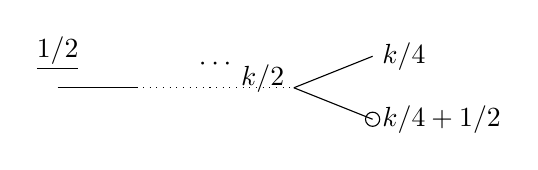
\begin{tikzpicture}[baseline=-2pt,x=1cm]
\draw(0,0)--(1,0);\draw[dotted](1,0)--(3,0);\draw(3,0)--(4,.4);\draw(3,0)--(4,-.4);\draw(4,-.4)circle(.09);\node[above]at(0,.1){$\underline{1/2}$};\node[above]at(2,.1){$\cdots$};\node[left]at(3,.12){$k/2$};\node[right]at(4,.4){$k/4$};\node[right]at(4,-.4){$k/4+1/2$};
\end{tikzpicture}\quad$(k+2\ge5)$\\[7pt]
$E_6$ &
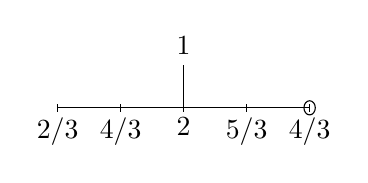
\begin{tikzpicture}[baseline=-2pt,x=.8cm]
\draw(0,0)--(4,0);\draw(2,0)--(2,.55);\foreach \x/\a in {0/{2/3},1/{4/3},2/{2},3/{5/3},4/{4/3}}{\draw(\x,-.05)--(\x,.05);\node[below]at(\x,0){$\a$};}\node[above]at(2,.55){$1$};\draw(4,0)circle(.09);
\end{tikzpicture}\\[7pt]
$E_7$ &
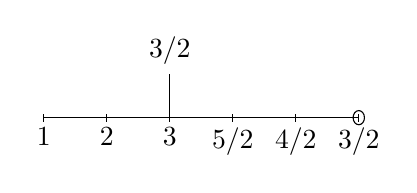
\begin{tikzpicture}[baseline=-2pt,x=.8cm]
\draw(0,0)--(5,0);\draw(2,0)--(2,.55);\foreach \x/\a in {0/{1},1/{2},2/{3},3/{5/2},4/{4/2},5/{3/2}}{\draw(\x,-.05)--(\x,.05);\node[below]at(\x,0){$\a$};}\node[above]at(2,.55){$3/2$};\draw(5,0)circle(.09);
\end{tikzpicture}
\end{tabular}
\end{center}
\end{minipage}\par
\paragraph*{1.3.10. 注。} (i) $G$ 为例外单群时，没有满足1.3.2的 $W$。

(ii) $G$ 为经典单群时，除 $D_l^{\mathbb H}$（$l\ge5$）外，这些 $W$ 组成 $\widetilde G$ 的忠实表示系。对 $D^{\mathbb H}$，只能得到 $G$ 的二重覆盖的忠实表示，即带非退化反 Hermitian 形式的四元数向量空间的自同构群的代数连通分支，这是 $\operatorname{SO}(2n)$ 的内形式。

\origsection{2}{Shimura 簇（Variétés de Shimura）}
\origsubsection{2.0}{预备知识（Préliminaires）}
\paragraph*{2.0.1.} 设 $G$ 为群，$\Gamma\subset G$，$\varphi:\Gamma\to\Delta$ 为同态，且给定 $\Delta$ 在 $G$ 上保持 $\Gamma$ 的作用 $r$，满足：(a) $r(\varphi(\gamma))=\operatorname{int}_\gamma$；(b) $\varphi$ 对 $\Delta$ 在 $\Gamma$ 上的 $r$ 作用与自身内自同构作用等变，即 $\varphi(r(\delta)(\gamma))=\operatorname{int}_\delta(\varphi(\gamma))$。

形成半直积 $G\rtimes\Delta$。条件等价于 $\{\gamma\varphi(\gamma)^{-1}\}$ 为正规子群，以其商定义 $G*_{\Gamma}\Delta$。由假设，$Z=\ker\varphi$ 在 $G$ 中心，$\operatorname{Im}\varphi$ 在 $\Delta$ 中正规。下图两行正合：
\begin{equation}
 \begin{tikzcd}[column sep=small]
 0\arrow[r]&Z\arrow[r]\arrow[d,equal]&\Gamma\arrow[r]\arrow[d]&\Delta\arrow[r]\arrow[d]&\Delta/\Gamma\arrow[r]\arrow[d,equal]&0\\
 0\arrow[r]&Z\arrow[r]&G\arrow[r]&G*_{\Gamma}\Delta\arrow[r]&\Delta/\Gamma\arrow[r]&0.
 \end{tikzcd}
 \tag{2.0.1.1}
\end{equation}
因此有同构
\begin{equation}
 \Gamma\backslash G\xrightarrow{\sim}\Delta\backslash(G*_{\Gamma}\Delta).
 \tag{2.0.1.2}
\end{equation}
由此得到 $G*_{\Gamma}\Delta$ 在 $\Gamma\backslash G$ 上的右作用：$G$ 按右平移，$\Delta$ 按右作用 $r^{-1}$。

若 $G$ 拓扑群、$\Delta$ 离散、$r$ 连续，则赋商拓扑的 $G*_{\Gamma}\Delta$ 为拓扑群，$G/\ker\varphi$ 为其开子群，(2.0.1.2)为同胚。这一构造同样适用于域上的代数群范畴。对约化 $k$ 群，有典范同构 $G=\widetilde G*_{Z(\widetilde G)}Z(G)$，其中 $Z(G)$ 对 $\widetilde G$ 平凡作用。
\paragraph*{2.0.2.} 设 $G$ 为 $k$ 代数群，中心为 $Z$，商为 $G^{\mathrm{ad}}$。内共轭映射 $(x,y)\mapsto xyx^{-1}$ 在 $Z\times\{e\}$ 的平移下不变，故经 $G^{\mathrm{ad}}$ 作用分解。注意 $G^{\mathrm{ad}}(k)$ 元素在 $G(k)$ 上未必为内自同构，因为 $G(k)\to G^{\mathrm{ad}}(k)$ 未必满；典型例子为 $\operatorname{PGL}(n,k)$ 对 $\SL(n,k)$ 的作用。同样，交换子（commutator）映射 $(x,y)\mapsto xyx^{-1}y^{-1}$ 对 $Z\times Z$ 平移不变，因而经映射 $(\ ,\ ):G^{\mathrm{ad}}\times G^{\mathrm{ad}}\to G$ 分解。

这些构造以及交换子、内自同构所满足的通常恒等式，都可借助下降（descent）得到清楚的解释：把 $G$ 看作适当景（site）上的群层，$G^{\mathrm{ad}}$ 看作模其中心的商层。特征零且只关心域扩张上的点时，Galois 下降已足够，参见2.4.1、2.4.2。

\emph{变体。} 约化 $G$ 与 $\widetilde G$ 有相同伴随群，以上构造相容。特别地，交换子有典范分解
\[
 G\times G\longrightarrow G^{\mathrm{ad}}\times G^{\mathrm{ad}}
 \longrightarrow\widetilde G\longrightarrow G.
\]
所以 $G(k)/\rho\widetilde G(k)$ 阿贝尔。
\paragraph*{2.0.3.} 设 $k$ 为特征零整体域，$A$ 为阿代尔环，$G$ 半单，$N=\ker(\rho:\widetilde G\to G)$。对有限个位组成的集合 $S$，以 $A_S$ 表示 $S$ 阿代尔，即在 $v\notin S$ 上的限制积。令
\[
 \Gamma_S=\rho\widetilde G(A_S)\cap G(k)\quad\text{（在 }G(A_S)\text{ 中相交）}.
\]
它由那些在每个 $v\notin S$ 都可提升到 $\widetilde G(k_v)$ 的有理元素组成；回忆 $\rho:\widetilde G(A)\to G(A)$ 固有。

上同调长正合列将 $G(k)/\rho\widetilde G(k)$ 识别为 $H^1(\Gal(\bar k/k),N(\bar k))$ 的子群，将 $\Gamma_S/\rho\widetilde G(k)$ 识别为此子群中在 $S$ 外局部为零者。特别地，它包含于 $H_*^1(\Gal(\bar k/k),N(\bar k))$，这里下标表示在每个单生成子群上的限制为零，论证和记号见 [12]。若 $\operatorname{Im}\Gal(\bar k/k)$ 为 Galois 在 $\Aut N(\bar k)$ 中的像，则
\[
 H_*^1(\Gal(\bar k/k),N(\bar k))
 =H_*^1(\operatorname{Im}\Gal(\bar k/k),N(\bar k)).
\]
特别地，$\Gamma_S/\rho\widetilde G(k)$ 有限。
\begin{originaltheorem}{命题 2.0.4}
(i) $\Gamma_S$ 只依赖于 $S$ 中分解群 $D_v\subset\operatorname{Im}\Gal(\bar k/k)$ 非循环的位；特别地加入无穷位不改变它。

(ii) $\Gamma_S/\rho\widetilde G(k)$ 识别为有限群 $H_*^1(\operatorname{Im}\Gal(\bar k/k),N(\bar k))$ 中在每个 $D_v$（$v\notin S$）上限制为零的类。$S$ 足够大时，二者相等。
\end{originaltheorem}
\begin{proof}
$H_*^1$ 的元素在循环分解群上的限制自动为零，得(i)。证明(ii)可假设 $S$ 含无穷位。$\widetilde G$ 对来自中心的类满足 Hasse 原理，保证(ii)中所有元素确实可实现为障碍类。
\end{proof}
\begin{originaltheorem}{推论 2.0.5}
$G(k)$ 的足够小的 $S$ 同余子群均包含在 $\Gamma_S$ 中。
\end{originaltheorem}
若 $U$ 为 $S$ 同余子群，$U/(U\cap\rho\widetilde G(k))$ 有限：提升障碍在次数和分歧有界的 Galois 扩张中消失，因此位于某个有限 Galois 商的 $H^1$ 中。适当的 $S$ 同余条件可从此 $H^1$ 降到 $\Gamma_S/\rho\widetilde G(k)$，见 [12]。
\paragraph*{2.0.6. 注。} 若 $\widetilde G$ 满足相对于 $S$ 的强逼近，则每个 $S$ 同余子群 $U\subset\Gamma_S$ 都满射到 $\Gamma_S/\rho\widetilde G(k)$。
\begin{originaltheorem}{推论 2.0.7}
对每个阿基米德位 $v$，足够小的 $S$ 同余子群 $U\subset G(k)$ 都位于 $G(k_v)$ 的拓扑中性分支内。
\end{originaltheorem}
因 $\widetilde G(k_v)$ 连通，有 $G(k_v)^+=\rho\widetilde G(k_v)$，且由2.0.4、2.0.5，$U\subset\Gamma_S=\Gamma_{S\cup\{v\}}\subset G(k_v)^+$。
\begin{originaltheorem}{推论 2.0.8}
$G(A_S)$ 的子群 $G(k)\rho\widetilde G(A_S)$ 闭，且拓扑同构于 $\rho\widetilde G(A_S)*_{\Gamma_S}G(k)$，即前者为其开子群。
\end{originaltheorem}
\begin{proof}
由2.0.2，$\rho\widetilde G(A_S)$ 正规且商交换，故所述集合确为子群。取足够大 $T\supset S$，使 $\widetilde G(k)$ 在 $\widetilde G(A_T)$ 中稠密。以 $k_{T-S}$ 表示对应局部域的乘积。对 $G(A_T)$ 的紧开子群 $K$，
\[
 \begin{split}
 G(k)\rho\widetilde G(A_S)
 &=G(k)\rho\bigl(\widetilde G(k)\widetilde G(k_{T-S})\times\rho^{-1}K\bigr)\\
 &\subset G(k)\bigl(\rho\widetilde G(k_{T-S})\times K\bigr).
 \end{split}
\]
由2.0.5，当 $K$ 够小时，在 $G(A_T)$ 内有 $G(k)\cap K\subset\Gamma_T$，所以在 $G(A_S)$ 内
\[
 G(k)\cap(\rho\widetilde G(k_{T-S})\times K)\subset\Gamma_S\subset\rho\widetilde G(A_S).
\]
于是所述群与开子群 $\rho\widetilde G(k_{T-S})\times K$ 的交包含于 $\rho\widetilde G(A_S)$，推论成立。
\end{proof}
\begin{originaltheorem}{推论 2.0.9}
若 $\widetilde G$ 满足相对于 $S$ 的强逼近，则 $G(k)$ 在 $G(A_S)$ 中的闭包为 $G(k)\rho\widetilde G(A_S)$。
\end{originaltheorem}
\paragraph*{2.0.10.} 设 $T$ 为 $k$ 环面，有限 $S$ 含所有阿基米德位，$U\subset T(k)$ 为 $S$ 单位群（$S$-units）。Chevalley 定理指出，$U$ 的每个有限指数子群都是同余子群，优美证明见 [12]。因此环面同源 $T'\to T$ 将同余子群映为同余子群。
\paragraph*{2.0.11.} 设 $G$ 约化，$\rho:\widetilde G\to G^{\mathrm{der}}$ 为万有覆盖，中心为 $Z$，中性分支 $Z^0$。以下为2.0.10的几个推论，均假定 $S$ 含阿基米德位。
\begin{originaltheorem}{推论 2.0.12}
若 $U$ 在 $Z(k)$ 的 $S$ 单位群中指数有限，则存在 $G(A_S)$ 的紧开子群 $K$，使
\[
 G(k)\cap(KG^{\mathrm{der}}(A_S))\subset G^{\mathrm{der}}(k)U.
\]
\end{originaltheorem}
将2.0.10应用于同源 $Z^0\to G/G^{\mathrm{der}}$：$K$ 够小时，$\gamma\in G(k)\cap KG^{\mathrm{der}}(A_S)$ 在阿贝尔化中的像对 $S$ 同余拓扑足够小，可提升为 $Z(k)$ 中足够小的 $z$，然后写 $\gamma=(\gamma z^{-1})z$。
\begin{originaltheorem}{推论 2.0.13}
$G^{\mathrm{der}}$ 的同余子群与 $Z^0(k)$ 的 $S$ 单位群的有限指数子群之积，是 $G(k)$ 的 $S$ 同余子群。
\end{originaltheorem}
\begin{originaltheorem}{推论 2.0.14}
$G(k)$ 的足够小的 $S$ 同余子群包含于 $G(\R)^+$。
\end{originaltheorem}
对 $G^{\mathrm{der}}$ 应用2.0.13、2.0.7，对 $Z^0$ 应用2.0.10即可。
\paragraph*{2.0.15.} $G^{\mathrm{der}}(k)\rho\widetilde G(A)$ 在 $G(k)\rho\widetilde G(A)$ 中开，因为它是离散群 $G(k)/G^{\mathrm{der}}(k)$ 的单位元逆像；该离散群包含在 $(G/G^{\mathrm{der}})(A)$ 中。由2.0.8，$G(k)\rho\widetilde G(A)$ 在 $G(A)$ 中闭。令
\begin{equation}
 \pi(G)=G(A)/G(k)\rho\widetilde G(A).
 \tag{2.0.15.1}
\end{equation}
由2.0.2的交换子构造，$G^{\mathrm{ad}}(k)$ 诱导在 $\pi(G)$ 上的作用平凡。

\origsubsection{2.1}{Shimura 簇（Variétés de Shimura）}
\paragraph*{2.1.1.} 设 $G$ 为 $\Q$ 上约化群，$X$ 为实代数群同态 $\mathbb S\to G_{\R}$ 的 $G(\R)$ 共轭类。假设以下公理：
\begin{enumerate}
\item[(2.1.1.1)] 对 $h\in X$，$\Lie(G_{\R})$ 类型为 $\{(-1,1),(0,0),(1,-1)\}$。
\item[(2.1.1.2)] $\operatorname{int}h(i)$ 为 $G_{\R}^{\mathrm{ad}}$ 的 Cartan 对合。
\item[(2.1.1.3)] $G^{\mathrm{ad}}$ 不存在定义于 $\Q$ 的因子，使 $h$ 在该因子上的投影平凡。
\end{enumerate}
第一条使 $w_h$ 取值于中心，因此与 $h$ 无关，记 $w_X$ 或 $w$。若进一步假设下列条件，会有若干简化：
\begin{enumerate}
\item[(2.1.1.4)] $w:\Gm\to G_{\R}$ 定义于 $\Q$；
\item[(2.1.1.5)] $\operatorname{int}h(i)$ 为 $(G/w(\Gm))_{\R}$ 的 Cartan 对合。
\end{enumerate}
由1.1.14(i)，$X$ 有唯一复结构，使每个表示的 Hodge 滤过全纯变化，且各连通分支为 Hermitian 对称域。1.1.17的证明也表明，$h$ 在 $G_{\R}^{\mathrm{ad}}$ 的紧单因子上平凡，每个分支为对应非紧因子的对称域乘积。第三公理等价于 $G^{\mathrm{ad}}$，或 $\widetilde G$，没有 $\Q$ 因子 $G'$ 使 $G'(\R)$ 紧；强逼近因此保证 $\widetilde G(\Q)$ 在 $\widetilde G(A^f)$ 中稠密。
\paragraph*{2.1.2.} Shimura 簇 ${}_KM_{\C}(G,X)$，简称 ${}_KM_{\C}$，为
\[
 {}_KM_{\C}(G,X)=G(\Q)\backslash\bigl(X\times(G(A^f)/K)\bigr),
\]
其中 $K$ 遍历紧开子群。由1.2.7及0.3，$\pi_0(X)$ 是 $G(\R)/G(\R)_+$ 的主齐性空间。实逼近使 $G(\Q)$ 在 $G(\R)$ 中稠密，因此 $G(\Q)/G(\Q)_+\cong G(\R)/G(\R)_+$。固定连通分支 $X^+$ 后，
\[
 {}_KM_{\C}=G(\Q)_+\backslash\bigl(X^+\times(G(A^f)/K)\bigr).
\]
它是以有限双陪集 $G(\Q)_+\backslash G(A^f)/K$ 为指标的商 $\Gamma_g\backslash X^+$ 的不交并。这里 $\Gamma_g$ 是 $\Gamma'_g=gKg^{-1}\cap G(\Q)_+$ 在 $G^{\mathrm{ad}}(\R)^+$ 中的像。这些群都是算术子群，因而相应的商具有自然的解析空间结构。

[2] 赋予这些商自然的拟射影代数簇结构（quasi-projective algebraic variety），因而 ${}_KM_{\C}$ 也具有这种结构。当 $K$ 足够小时，各 $\Gamma_g$ 都无挠；由 [3]，此时上述代数结构唯一。更精确地，对任意既约概形 $Z$，从 $Z$ 到该商的解析态射自动代数。
\paragraph*{2.1.3.} 有
\[
 \begin{split}
 \pi_0({}_KM_{\C})
 &=G(\Q)\backslash\bigl(\pi_0(X)\times G(A^f)/K\bigr)\\
 &=G(\Q)\backslash G(A)/(G(\R)_+\times K)
 =G(\Q)_+\backslash G(A^f)/K.
 \end{split}
\]
因 $G(A^f)/K$ 离散，可用闭包 $G(\Q)_+^-$ 代替 $G(\Q)_+$。$\widetilde G(\R)$ 连通，故 $\rho\widetilde G(\Q)\subset G(\Q)_+$；强逼近使其在 $\rho\widetilde G(A^f)$ 中稠密。因此
\begin{equation}
 \begin{split}
 \pi_0({}_KM_{\C})
 &=G(\Q)_+\rho\widetilde G(A^f)\backslash G(A^f)/K\\
 &=G(A^f)/(\rho\widetilde G(A^f)G(\Q)_+K)
 =G(A^f)/(G(\Q)_+^-K),
 \end{split}
 \tag{2.1.3.1}
\end{equation}
因为 $\rho\widetilde G(A^f)$ 正规且商阿贝尔。类似地，令 $\bar\pi_0\pi(G)=\pi_0\pi(G)/\pi_0G(\R)_+$，则
\begin{equation}
 \begin{split}
 \pi_0({}_KM_{\C})
 &=G(A)/(\rho\widetilde G(A)G(\Q)(G(\R)_+\times K))\\
 &=\pi(G)/(G(\R)_+\times K)=\bar\pi_0\pi(G)/K.
 \end{split}
 \tag{2.1.3.2}
\end{equation}
特别地，只依赖 $K$ 在 $G(A)/\rho\widetilde G(A)$ 中的像。
\paragraph*{2.1.4.} 随 $K$ 缩小，各 ${}_KM_{\C}$ 形成投射系统，具有 $G(A^f)$ 的右作用，即同构 $g:{}_KM_{\C}\to{}_{g^{-1}Kg}M_{\C}$。更方便的是考虑概形 $M_{\C}(G,X)=\operatorname{proj\,lim}_K{}_KM_{\C}$。转移态射有限，故极限存在。它带右作用，且模 $K$ 得回原簇。下面确定该概形及其连通分解。
\begin{originaltheorem}{定义 2.1.5}
固定 $X$ 的连通分支 $X^+$。$M_{\C}$ 的中性分支 $M_{\C}^0$ 为包含 $X^+\times\{e\}\subset X\times G(A^f)$ 的像的连通分支。
\end{originaltheorem}
\begin{originaltheorem}{定义 2.1.6}
设 $G_0$ 为 $\Q$ 伴随群，无使实点紧的 $\Q$ 因子，$G_1$ 为其覆盖。以 $\tau(G_1)$ 表示 $G_0(\Q)$ 上由 $G_1(\Q)$ 的同余子群的像作为单位元基本邻域系的拓扑。
\end{originaltheorem}
以 $\wedge(\mathrm{rel.}\ G_1)$ 或简单 $\wedge$ 表示此拓扑下的完备化。令 $\rho:\widetilde G_0\to G_1$ 为自然映射，$\Gamma=\rho\widetilde G_0(A)\cap G_1(\Q)$，上横线表示在 $G_1(A^f)$ 的闭包。因 $\widetilde G_0(\R)$ 连通，$\Gamma\subset G_1(\Q)^+$。由2.0.9、2.0.14，
\begin{equation}
 G_0(\Q)^\wedge(\mathrm{rel.}\ G_1)
 =G_1(\Q)^-*_{G_1(\Q)}G_0(\Q)
 =\rho\widetilde G_0(A^f)*_\Gamma G_0(\Q),
 \tag{2.1.6.1}
\end{equation}
\begin{equation}
 G_0(\Q)^{+\wedge}(\mathrm{rel.}\ G_1)
 =G_1(\Q)_+^-*_{G_1(\Q)_+}G_0(\Q)^+
 =\rho\widetilde G_0(A^f)*_\Gamma G_0(\Q)^+.
 \tag{2.1.6.2}
\end{equation}
\begin{originaltheorem}{命题 2.1.7}
$M_{\C}^0$ 为 $\Gamma\backslash X^+$ 的投射极限，其中 $\Gamma\subset G^{\mathrm{ad}}(\Q)^+$ 遍历对 $\tau(G^{\mathrm{der}})$ 开的算术子群。
\end{originaltheorem}
由2.1.2，它是 $G(\Q)_+$ 同余子群的像所对应的商的极限；由2.0.13，可用 $G^{\mathrm{der}}$ 代替 $G$。
\paragraph*{2.1.8.} 投影 $G\to G^{\mathrm{ad}}$ 将 $X^+$ 同构到 $\mathbb S\to G_{\R}^{\mathrm{ad}}$ 的某个 $G(\R)^+$ 共轭类。由2.1.7，中性分支只依赖 $G^{\mathrm{ad}},G^{\mathrm{der}}$ 及这个共轭类。具体表述如下：设 $G$ 伴随，$X^+$ 满足前三公理，$G_1$ 为覆盖。连通 Shimura 簇（connected Shimura varieties）指所有商 $\Gamma\backslash X^+$，其中 $\Gamma\subset G(\Q)^+$ 算术且对 $\tau(G_1)$ 开。其投射极限记为 $M_{\C}^0(G,G_1,X^+)$。结构搬运给出的 $G(\Q)^+$ 作用连续延拓到完备化 $G(\Q)^{+\wedge}(\mathrm{rel.}\ G_1)$ 的作用。采用此前识别，有
\[
 M_{\C}^0(G,X)=M_{\C}^0(G^{\mathrm{ad}},G^{\mathrm{der}},X^+).
\]
\paragraph*{2.1.9.} 设 $Z$ 为中心，$Z(\Q)^-$ 为其在 $Z(A^f)$ 中的闭包。由 Chevalley（2.0.10），这就是 $Z(\Q)$ 对单位群有限指数子群拓扑的完备化，也等于它在 $\pi_0Z(\R)\times Z(A^f)$ 中的闭包。

对紧开 $K$，$Z(\Q)K=Z(\Q)^-K$，故
\[
 \begin{split}
 {}_KM_{\C}
 &=G(\Q)\backslash(X\times G(A^f)/K)\\
 &=(G(\Q)/Z(\Q))\backslash(X\times G(A^f)/(Z(\Q)K))\\
 &=(G(\Q)/Z(\Q))\backslash(X\times G(A^f)/(Z(\Q)^-K)).
 \end{split}
\]
$G(\Q)/Z(\Q)$ 在 $X\times G(A^f)/Z(\Q)^-$ 上的作用固有，因此可对 $K$ 取极限：
\begin{originaltheorem}{命题 2.1.10}
$M_{\C}(G,X)=(G(\Q)/Z(\Q))\backslash(X\times G(A^f)/Z(\Q)^-)$。
\end{originaltheorem}
\begin{originaltheorem}{推论 2.1.11}
若2.1.1.4及2.1.1.5成立，则 $M_{\C}(G,X)=G(\Q)\backslash(X\times G(A^f))$。
\end{originaltheorem}
因为此时 $Z(\Q)$ 在 $Z(A^f)$ 中离散，闭包即自身。
\begin{originaltheorem}{推论 2.1.12}
右作用经 $G(A^f)/Z(\Q)^-$ 分解。
\end{originaltheorem}
\paragraph*{2.1.13.} 以 $G^{\mathrm{ad}}(\R)_1$ 表示 $G(\R)$ 的像，$G^{\mathrm{ad}}(\Q)_1=G^{\mathrm{ad}}(\Q)\cap G^{\mathrm{ad}}(\R)_1$。2.0.2的作用诱导它在系统上的左作用
\[
 \operatorname{int}(\gamma):{}_KM_{\C}\xrightarrow{\sim}{}_{\gamma K\gamma^{-1}}M_{\C},
\]
以及极限上的作用。$\gamma\in G^{\mathrm{ad}}(\Q)^+$ 时保持中性分支，从而保持全部分支，并在其上诱导2.1.6的作用。
将此作用转换成右作用，记 $\cdot\gamma$。若 $\gamma$ 为 $\delta\in G(\Q)$ 的像，此右作用等于把 $\delta$ 视为 $G(A^f)$ 元素的右作用。事实上，若 $u$ 为 $(x,g)$ 的像，$u\cdot\gamma$ 为
\[
 (\gamma^{-1}x,\operatorname{int}_\gamma^{-1}g)
 =(\delta^{-1}x,\delta^{-1}g\delta)\sim(x,g\delta)
\]
的像，其中最后在左侧模 $G(\Q)$。总之得到下列群的右作用：
\begin{equation}
 \frac{G(A^f)}{Z(\Q)^-}*_{G(\Q)/Z(\Q)}G^{\mathrm{ad}}(\Q)_1
 =\frac{G(A^f)}{Z(\Q)^-}*_{G(\Q)_+/Z(\Q)}G^{\mathrm{ad}}(\Q)^+.
 \tag{2.1.13.1}
\end{equation}
\begin{originaltheorem}{命题 2.1.14}
$G(A^f)$ 的右作用使 $\pi_0M_{\C}$ 成为阿贝尔商 $G(A^f)/G(\Q)_+^-\allowbreak=\bar\pi_0\pi(G)$ 的主齐性空间。
\end{originaltheorem}
这是2.1.3公式取极限的直接结果。
\paragraph*{2.1.15.} 因 $G^{\mathrm{ad}}(\Q)$ 在 $\pi(G)$ 上平凡，而 $G^{\mathrm{ad}}(\Q)^+$ 至少稳定一个分支，故稳定全部分支。因此(2.1.13.1)作用中，每个分支的稳定子为
\begin{equation}
 \frac{G(\Q)_+^-}{Z(\Q)^-}*_{G(\Q)_+/Z(\Q)}G^{\mathrm{ad}}(\Q)^+
 =G^{\mathrm{ad}}(\Q)^{+\wedge}(\mathrm{rel.}\ G^{\mathrm{der}}),
 \tag{2.1.15.1}
\end{equation}
其中等式来自2.0.13。
\paragraph*{2.1.16. 小结。} 群(2.1.13.1)右作用于 $M_{\C}$。其模 $G^{\mathrm{ad}}(\Q)^+$ 闭包的阿贝尔商为
\[
 G(A^f)/G(\Q)_+^-=\bar\pi_0\pi(G).
\]
投有限集（profinite set）$\pi_0M_{\C}$ 为此商的主齐性空间。该闭包是对导出群同余子群像拓扑的完备化；它在中性分支上的作用，转换为左作用后就是2.1.8的作用。

\origsubsection{2.2}{典范模型（Modèles canoniques）}
\paragraph*{2.2.1.} 设 $(G,X)$ 如2.1.1。$h\in X$ 对应 $\mu_h:\Gm\to G_{\C}$（1.1.1、1.1.11）。其共轭类的定义域称为 $(G,X)$ 的对偶域（reflex field）$E(G,X)\subset\C$。固定连通分支 $X^+$ 后，也记为 $E(G,X^+)$。若 $f:G'\to G''$ 将 $X'$ 映入 $X''$，则 $E(G',X')\supset E(G'',X'')$。
\paragraph*{2.2.2.} 设 $T$ 为环面，$E$ 为数域，$\mu:\Gm\to T_E$ 定义于 $E$。将 $E^\times$ 视为 $\Q$ 群 $R_{E/\Q}\Gm$，对 $\mu$ 作限制得到 $R_{E/\Q}(\mu):E^\times\to R_{E/\Q}T_E$。再复合范数映射 $N_{E/\Q}:R_{E/\Q}T_E\to T$（有理点上即 $T(E)\to T(\Q)$），得到 $NR_E(\mu)$，或简称 $NR(\mu)$。扩张 $E'/E$ 后有
\begin{equation}
 NR_{E'}(\mu)=NR_E(\mu)\circ N_{E'/E}.
 \tag{2.2.2.1}
\end{equation}
\paragraph*{2.2.3.} 特别设 $h:\mathbb S\to T_{\R}$，$X=\{h\}$。若 $E\supset E(T,X)$，则 $\mu_h$ 定义于 $E$。由 $NR(\mu_h)$ 对阿代尔点取模有理点，得到 $C(E)\to T(\Q)\backslash T(A)$，再取连通分支得到
\[
 \pi_0NR(\mu_h):\pi_0C(E)\to\pi_0(T(\Q)\backslash T(A)).
\]
整体类域论将源识别为 $E$ 的阿贝尔化 Galois 群。目标为投有限群，是 $T(\Q)\backslash T(A)/\allowbreak(T(\R)^+\times K)$ 的极限，也等于 $(\pi_0T(\R)\times T(A^f))/\allowbreak T(\Q)^-$。环面的 Shimura 簇为有限集 $T(\Q)\backslash T(A^f)/K$，其极限 $T(A^f)/T(\Q)^-$ 是该目标模 $\pi_0T(\R)$。

定义互反态射（reciprocity morphism）
\[
 r_E(T,X):\Gal(\overline\Q/E)^{\mathrm{ab}}\to T(A^f)/T(\Q)^-
\]
为对如下复合逐点取群逆所得的同态：0.8的类域论同构、$\pi_0NR(\mu_h)$、向有限阿代尔商的投影。它给出 Galois 在各 ${}_KM_{\C}(T,X)$ 上的作用：$\sigma$ 按 $r_E(T,X)(\sigma)$ 右平移。普遍情形为 $E=E(T,X)$；由2.2.2.1，一般 $r_E$ 是该作用在 $\Gal(\overline\Q/E)$ 上的限制。
\paragraph*{2.2.4.} 点 $h\in X$ 若经定义于 $\Q$ 的环面 $T\subset G$ 分解，称为特殊（special），或 CM 型（CM type）。Cartan 对合在 $T(\R)$ 于伴随群中的像上平凡，该像因此紧。$E(T,\{h\})$ 只依赖 $h$，记为 $E(h)$。

对 ${}_KM_{\C}$ 或 $M_{\C}$ 的点 $x=[h,g]$，$h$ 的 $G(\Q)$ 共轭类仅依赖 $x$。若 $h$ 特殊，称 $x$ 特殊，$E(x)=E(h)$ 称为其对偶域，该共轭类称为 $x$ 的类型（type）。

在固定类型、对偶域为 $E$ 的特殊点集上定义 Galois 作用如下。取点 $x=[h,g]$，使 $h$ 经有理环面 $T$ 分解，$\sigma\in\Gal(\overline\Q/E)$，并在 $T(A^f)$ 取 $r_E(T,\{h\})(\sigma)$ 的代表元 $\widetilde r(\sigma)$。令
\[
 r(\sigma)x=[h,\widetilde r(\sigma)g].
\]
可验证只依赖 $x,\sigma$，且与 $G(A^f)$ 右作用交换。
\paragraph*{2.2.5.} $M_{\C}(G,X)$ 的典范模型是其在 $E(G,X)$ 上、带 $G(A^f)$ 右作用的形式 $M(G,X)$，满足：(a) 特殊点为代数点；(b) 对给定类型 $\tau$、对偶域 $E(\tau)$ 的特殊点，$\Gal(\overline\Q/E(\tau))\subset\Gal(\overline\Q/E(G,X))$ 按2.2.4作用。

“形式”指带右作用的 $E(G,X)$ 概形 $M$，及等变同构 $M\otimes_{E(G,X)}\C\cong M_{\C}$。若数域 $E\subset\C$ 包含对偶域，$E$ 上的弱典范模型是相同的 $E$ 形式，满足(a)以及(b$^*$)：将(b)的 Galois 群换为 $\Gal(\overline\Q/E(\tau))\cap\Gal(\overline\Q/E)$。
\paragraph*{2.2.6.} [5，5.4、5.5] 借鉴 Shimura 方法，证明 $M_{\C}(G,X)$ 在 $E$ 上至多有一个弱典范模型；若存在，则对 $(G,X)$ 函子化。

\origsubsection{2.3}{典范模型的构造（Construction de modèles canoniques）}
本节确定下列 [5，4.21、5.7] 判据的适用情形。
\begin{originaltheorem}{判据 2.3.1}
设 $(G,X)$ 如2.1.1，有理向量空间 $V$ 带非退化反对称形式 $\Psi$，$S^\pm$ 为相应双 Siegel 半空间（1.3.1）。若存在嵌入 $G\hookrightarrow\operatorname{CSp}(V)$ 将 $X$ 映入 $S^\pm$，则 $M_{\C}(G,X)$ 有典范模型。
\end{originaltheorem}
\begin{originaltheorem}{命题 2.3.2}
设 $w=w_h$，$(V,\rho)$ 为 $G$ 的类型 $\{(-1,0),(0,-1)\}$ 的忠实表示。若 $\operatorname{int}h(i)$ 为 $G_{\R}/w(\Gm)$ 的 Cartan 对合，则存在反对称形式 $\Psi$ 使 $\rho$ 诱导 $(G,X)\hookrightarrow(\operatorname{CSp}(V),S^\pm)$。
\end{originaltheorem}
按假设 $V$ 纯权 $-1$，故 $w$ 定义于 $\Q$，取1.1.18(b)的有理极化形式即可。
\begin{originaltheorem}{推论 2.3.3}
设 $V$ 为上述类型的忠实表示。若连通中心 $Z^0$ 在 CM 型域（CM field）上分裂，则存在与 $G$ 具有相同导出群、且 $X$ 经之分解的子群 $G_2$，以及 $V$ 上反对称形式 $\Psi$，使 $\rho$ 诱导 $(G_2,X)\hookrightarrow(\operatorname{CSp}(V),S^\pm)$。
\end{originaltheorem}
中心的假设等价于 $Z_{\R}^0$ 的极大紧子环面定义于 $\Q$。取由导出群、此环面及 $w$ 的像生成的 $G_2$，应用2.3.2。
\paragraph*{2.3.4.} 设 $G$ 为 $\Q$ 单伴随群。公理2.1.1.2保证 $G_{\R}$ 为其紧形式的内形式。这一点有以下两个推论。

(a) $G_{\R}$ 的单分量都绝对单。写作 Weil 限制 $G=R_{F/\Q}G^s$，$G^s$ 为 $F$ 上绝对单群，则 $F$ 全实。令 $I$ 为 $F$ 的实嵌入集，对 $v\in I$，$G_v=G^s\otimes_{F,v}\R$，$D_v$ 为其复化的 Dynkin 图。则 $G_{\R}=\prod G_v$，$G_{\C}=\prod G_{v\C}$，Dynkin 图 $D$ 为各 $D_v$ 的不交并。Galois 作用于 $D,I$，与投影 $D\to I$ 相容。

(b) 复共轭在 $D$ 上为对立对合，它在 $\Aut D$ 中心内。故 Galois 在图上的作用经有限忠实商 $\Gal(K_D/\Q)$ 分解；对立对合平凡时 $K_D$ 全实，否则为全实域的全虚二次扩张。
\paragraph*{2.3.5.} $X=\prod X_v$，各 $X_v$ 为 $\mathbb S\to G_v$ 的共轭类。紧 $G_v$ 的 $X_v$ 平凡；非紧时由特殊顶点 $s_v\in D_v$ 描述。令 $I_c$ 为紧位，$I_{nc}=I-I_c$；$D_c,D_{nc}$ 分别为对应图的并，$G_c,G_{nc}$ 为相应因子的积，覆盖也同样记。最后以 $\Sigma(X)$ 表示所有非紧位的 $s_v$ 组成的集合。
\begin{originaltheorem}{命题 2.3.6}
$(G,X)$ 的对偶域是 $K_D$ 中被 $\Gal(K_D/\Q)$ 内稳定 $\Sigma(X)$ 的子群固定的子域。
\end{originaltheorem}
\paragraph*{2.3.7.} 假设有图
\begin{equation}
 (G,X)\longleftarrow(G_1,X_1)\hookrightarrow(\operatorname{CSp}(V),S^\pm).
 \tag{2.3.7.1}
\end{equation}
$G$ 的万有覆盖提升到 $G_1$，故可将 $V$ 限制为 $\widetilde G$ 表示；忠实作用的商恰为 $G_1$ 的导出群。对
\[
 (G_{nc},X)\longleftarrow(\ker(G_{1\R}\to G_c)^0,X_1)
 \longrightarrow(\operatorname{CSp}(V),S^\pm)
\]
应用1.3.2、1.3.8，得 $\widetilde G_{nc\C}$ 表示的非平凡不可约分量均经一个 $\widetilde G_{v\C}$（$v\in I_{nc}$）分解，最高权为表1.3.9允许的基本权。整个 $\widetilde G_{\C}$ 表示的最高权集 Galois 稳定，因 Galois 在 $I$ 上传递且 $I_{nc}\ne\varnothing$，得到：

(a) $V_{\C}$ 的每个不可约分量 $W$ 都形如 $\bigotimes_{v\in T}W_v$，其中 $T\subset I$，$W_v$ 为基本表示，对应顶点 $\tau(v)\in D_v$。以 $\mathcal S(V)$ 表示这些 $\tau(T)\subset D$ 的集合。

(b) 对 $S\in\mathcal S(V)$，$S\cap D_{nc}$ 或空，或只有一点 $s_S\in D_v$。该点在对应 $(D_v,s_v)$ 的表1.3.9中为下划线顶点。

(c) $\mathcal S$ Galois 稳定，且不包含于 $\{\varnothing\}$。

对满足(b)、(c)的集合族，以 $\widetilde G(\mathcal S)_{\C}$ 表示在对应表示中忠实作用的商；由(c)它定义于 $\Q$。我们主要关心还满足下述条件的情形：(d) $\mathcal S$ 由单点子集组成。一般 $\mathcal S$ 可换成其中所有点的单点集合族 $\mathcal S'$，它满足(b)、(c)、(d)，且 $\widetilde G(\mathcal S')$ 覆盖 $\widetilde G(\mathcal S)$。

下表由1.3.9导出，列举存在(b)、(c)集合族的情形（只可能为经典 $A,B,C,D$ 型），并给出满足(b)、(c)、(d)的最大集合族及其商群；此群覆盖所有其余允许商群。
\paragraph*{表 2.3.8。}
\emph{$A,B,C$ 型。} 唯一集合族由各 $D_v$ 的端点对应的单点集组成，$B,C$ 取短根端点。覆盖为万有覆盖。

\emph{$D_l$ 型（$l\ge5$）。} 存在的充要条件是所有非紧 $(G_v,X_v)$ 同为 $D_l^{\R}$ 型，或同为 $D_l^{\mathbb H}$ 型。

$D_l^{\R}$：最大集合族取各图“右端”的单点集，覆盖为万有覆盖。

$D_l^{\mathbb H}$：唯一集合族取各图“左端”单点集，覆盖形如 $R_{F/\Q}\widetilde G^*$，其中 $\widetilde G^*$ 为 $G$ 的二重覆盖、$\operatorname{SO}(2l)$ 的形式，见1.3.10。

\emph{$D_4$ 型。} 以 $S=\{s:\{s\}\in\mathcal S\}$ 代替集合族，则(b)为 $S$ 包含于所有端点之集 $E$，并与 $\Sigma(X)$ 不交。具有此性质的最大 Galois 稳定子集是 $E-\Gal(\overline\Q/\Q)\Sigma(X)$。它与每个 $D_v$ 的交有0、1或2点。0点时不存在允许集合族；1或2点时，它自身或其补集为 Galois 不变截面 $\tau:I\to X$ 的像\footnote{\textbf{译者注（本次校订）：}此处截面的目标应为 $D$：$\tau$ 是投影 $D\to I$ 的截面，$\tau(v)$ 为 Dynkin 图 $D_v$ 的一个顶点。}，且分别与 $\Sigma(X)$ 不交或包含它。将 $\tau(v)$ 称为图的“左端”，即回到高秩情形。

$D_4^{\R}$：存在唯一截面 $\tau$ 使 $\tau(I)\supset\Sigma(X)$，其余同 $D_l^{\R}$。

$D_4^{\mathbb H}$：给定截面 $\tau$，像与 $\Sigma(X)$ 不交。若非上一情形，此截面唯一，唯一集合族由各左端单点集组成。覆盖为 $R_{F/\Q}\widetilde G^s$，其中 $\widetilde G^s$ 为由 $\tau$ 决定的二重覆盖。

此后约定 $D_4^{\mathbb H}$ 排除 $D_4^{\R}$。于是存在允许集合族当且仅当类型为 $A,B,C,D^{\R},D^{\mathbb H}$；除最后一型外，均可使其商为万有覆盖。
\paragraph*{2.3.9.} 取 $F$ 的全虚二次扩张 $K$，并选择复嵌入集 $T$，在每个 $v\in I_c$ 上恰取一个。它在视为有理向量空间的 $K$ 上定义 Hodge 结构 $h_T:\mathbb S\to K_{\R}^\times$：若 $J$ 为所有复嵌入，$K\otimes\C=\C^J$，则 $\sigma\in T$ 的因子类型为 $(-1,0)$，$\bar\sigma\in T$ 的为 $(0,-1)$，在 $I_{nc}$ 上方的为 $(0,0)$。主要结果如下。
\begin{originaltheorem}{命题 2.3.10}
设 $G$ 为 $\Q$ 单伴随群，类型为 $A,B,C,D^{\R},D^{\mathbb H}$。任取上述 $K,T$，存在图
\[
 (G,X)\longleftarrow(G_1,X_1)\hookrightarrow(\operatorname{CSp}(V),S^\pm),
\]
满足：(i) $E(G_1,X_1)$ 为 $E(G,X)$ 与 $E(K^\times,h_T)$ 的合成域；(ii) 前四型的 $G_1^{\mathrm{der}}$ 单连通，最后一型为2.3.8描述的覆盖。
\end{originaltheorem}
\begin{proof}
令 $S$ 为2.3.8确定的最大顶点集，单点族满足(b)、(c)。Galois 作用于 $S$，可将其识别为 $\Hom(K_S,\C)$，$K_S$ 为适当有限数域乘积，均同构于 $K_D$ 的子域，因固定 $K_D$ 的 Galois 群在 $D$ 从而在 $S$ 上平凡作用。故 $K_S$ 为全实或 CM 域的乘积。投影 $S\to I$ 对应 $F\to K_S$。

对 $s\in S$，取基本最高权表示 $V(s)$。$\bigoplus V(s)$ 的同构类定义于 $\Q$，但表示本身未必如此，障碍在适当 Brauer 群中；不过，总可以取足够多个同构副本，使其直和定义于 $\Q$。故取 $V$ 使 $V_{\C}\cong\bigoplus V(s)^n$，记其对应等型分量为 $V_s$。Galois 相容地置换分量，因此，这一分解赋予 $V$ 一个 $K_S$ 模结构，$K_S$ 在 $V_s$ 上经相应嵌入作数乘。令 $\widetilde G'$ 为忠实作用的商，即(ii)所需覆盖。

对 $h\in X$ 作到 $\widetilde G'_{\R}$ 的分数提升，在 $V$ 上得到权零分数 Hodge 结构。对 $s\mapsto v$，由表1.3.9：(a) 若 $v\in I_c$，$V_s$ 类型为 $(0,0)$；(b) 若 $v\in I_{nc}$，类型为 $\{(r,-r),(r-1,1-r)\}$，其中 $r$ 为图中特殊顶点 $s_v$ 所对应表项。

定义新的结构 $h_2$，保持紧位为 $(0,0)$，将非紧位的两个分量分别赋予类型 $(0,-1)$ 与 $(-1,0)$。令 $G_2\subset\GL(V)$ 为 $\widetilde G'$ 与 $K_S^\times$ 生成的群，则 $h_2:\mathbb S\to G_{2\R}$。记其共轭类为 $X_2$，有 $(G_2,X_2)\to(G,X)$，且 $E(G_2,X_2)=E(G,X)$。

在 $K\otimes_FV$ 上将 $V$ 的结构与2.3.9的 $K$ 的结构张量相乘，得 $h_3$。分解
\[
 (K\otimes_FV)\otimes\R
 =\bigoplus_{v\in I}(K\otimes_{F,v}\R)\otimes_{\R}(V\otimes_{F,v}\R)
\]
与 Hodge 结构相容。紧位上第一因子为 $\{(-1,0),(0,-1)\}$、第二因子为 $(0,0)$，非紧位反之。因此 $h_3$ 总为所需类型。令 $G_3$ 为 $K^\times$ 与 $G_2$ 生成的群，$X_3$ 为 $h_3$ 共轭类，则导出群为 $\widetilde G'$，且 $E(G_3,X_3)$ 为 $E(G,X)$ 与 $E(K^\times,h_T)$ 的合成。对 $(G_3,X_3)$ 及忠实表示应用2.3.3，得所需 $(G_1,X_1)$。
\end{proof}
\paragraph*{2.3.11. 注。} 此构造可推广到任意满足2.3.7(b)、(c)的集合族，使2.3.7.1中 $\mathcal S(V)=\mathcal S$。概括为：(a) 由 $\Hom(K_{\mathcal S},\C)=\mathcal S$ 定义代数，构造满足要求的 $V$，分解 $V_{\C}=\bigoplus V_S$ 给出其模结构；(b) 分数 Hodge 结构在紧位上方为 $(0,0)$，否则为由唯一非紧顶点决定的 $\{(r,-r),(r-1,1-r)\}$；(c) 将后者如上变换为 $\{(0,-1),(-1,0)\}$。
(d) 为将 $(0,0)$ 转成所需类型，在 $K_{\mathcal S}$ 上将 $V$ 与带适当 Hodge 结构 $h$ 的 CM 代数 $K'_{\mathcal S}$ 张量相乘。所得导出群为 $\widetilde G(\mathcal S)$，对偶域为 $E(G,X)$ 与 $E(K_{\mathcal S}'{}^\times,h)$ 的合成。即使满足(d)，此处处理 $(0,0)$ 的方法也比2.3.10更一般。
\paragraph*{2.3.12. 注。} 对特殊顶点被对立对合固定的 $A$ 型，以及 $B,C,D^{\R}$ 型，$E(G,X)$ 是 $K_D$ 中稳定 $I_c$ 的 Galois 子群的不动域，为全实域。若 $I_c=\varnothing$，即 $\Q$；若 $I_c$ 或 $I_{nc}$ 只有一点 $v$，则为 $v(F)$。$E(K,h_T)$ 都扩张此域。
\paragraph*{2.3.13. 注。} 对这些类型及 $D^{\mathbb H}$，2.3.10中非紧位的 $V_s$ 类型为 $\{(-1/2,1/2),(1/2,-1/2)\}$。因此可用 $F^\times$ 与 $\widetilde G'$ 生成的子群代替 $G_2$；若 $I_c=\varnothing$，甚至只需 $\Q^\times$。此时直接应用2.3.2，得到 $E(G_1,X_1)=E(G,X)$，除 $D^{\mathbb H}$ 外均等于 $\Q$。

\origsubsection{2.4}{互反律：预备知识（Lois de réciprocité : préliminaires）}
本节的构造将用于2.6，计算典范模型的互反律，即 Galois 群在几何连通分支集上的作用。本节采用非几何学家较熟悉的 Galois 下降。若使用 fppf 下降，表述本可更统一，并可省去某些重复以及可分性或特征零的假设。

设 $G$ 为整体域 $k$ 上约化群。采用2.0.15记号，目标是构造两类典范态射：(a) 对有限可分扩张 $k'/k$ 及 $G'=G\otimes_kk'$，构造范数
\begin{equation}
 N_{k'/k}:\pi(G')\longrightarrow\pi(G);
 \tag{2.4.0.1}
\end{equation}
(b) 对环面 $T$ 及定义于 $k$ 的 $T\to G$ 同态共轭类 $M$，构造
\begin{equation}
 q_M:\pi(T)\longrightarrow\pi(G).
 \tag{2.4.0.2}
\end{equation}
若 $m\in M(k)$，该映射就是 $m$ 所诱导的映射；关键在于证明它与 $m$ 的选择无关，并将构造推广到 $M$ 没有 $k$ 上代表的情形。函子性可直接由定义看出。
\paragraph*{2.4.1.} 系统使用挠子（torsors）的语言（我更喜欢它而非上循环语言），以及 Grothendieck 形式的 Galois 下降，见 SGA 1 或 SGA $4\frac12$［Arcata］。

\emph{Galois 下降。} 设 $K/k$ 有限可分。构造 $k$ 上对象 $X$（如挠子）时，只须：(a) 对每个容许 $K\to k'$ 的可分扩张 $k'/k$，构造 $X_{k'}$；(b) 对 $k''/k'$ 给出同构 $\chi_{k'',k'}:X_{k'}\otimes k''\cong X_{k''}$；(c) 验证复合相容性 $\chi_{k''',k''}\chi_{k'',k'}=\chi_{k''',k'}$。

在实际构造中，可以先在某个可分扩张 $K$ 上选取所需的辅助对象，再证明不同选择给出的 $X$ 之间存在唯一的相容同构。

\paragraph*{注1。} Galois 下降是平展（étale）局部化的特例；上述(a)、(b)、(c)构造常以“局部地”引入。
\paragraph*{例 2.4.2.} 解释2.0.2交换子映射的典范提升。采用 Galois 而非 fppf 下降，须假设 $G\to G^{\mathrm{ad}}$ 光滑，且只讨论点映射而非整个态射。对 $x_1,x_2\in G^{\mathrm{ad}}(k)$，可局部写 $x_i=\rho(\widetilde x_i)z_i$，$z_i$ 在中心。\footnote{\textbf{译者注（本次校订）：}此式的右侧属于 $G$，而 $x_i$ 原先属于 $G^{\mathrm{ad}}$。严格地说，应先在局部将 $x_i$ 提升为 $G$ 的元素，再作上述分解；不同提升相差中心元素，故所定义的交换子不受影响。}$\widetilde x_i$ 唯一至相差 $\widetilde G$ 中心元素，故其交换子与选择无关，定义 $(x_1,x_2)=\widetilde x_1\widetilde x_2\widetilde x_1^{-1}\widetilde x_2^{-1}$。
\paragraph*{2.4.3.} 对 $k$ 代数群 $G$，$G$ 挠子是带右 $G$ 作用、成为主齐性空间的 $k$ 概形 $P$。平凡挠子 $G_d$ 为带右平移作用的 $G$。点 $x\in P(k)$ 对应平凡化 $\varphi:G_d\cong P$，$\varphi(g)=xg$。

同态 $f:G_1\to G_2$ 及 $G_1$ 挠子 $P$ 给出一个在唯一同构意义下确定的 $G_2$ 挠子 $f(P)$，带映射 $f:P\to f(P)$ 满足 $f(pg)=f(p)f(g)$。记范畴 $[G_1\to G_2]$ 的对象为配有 $f(P)$ 平凡化的 $G_1$ 挠子；态射为与该平凡化相容的挠子同构。以 $H^0(G_1\to G_2)$ 表示 $(G_{1d},e)$ 的自同构群，即 $\ker(G_1(k)\to G_2(k))$；$H^1(G_1\to G_2)$ 为以该对象为基点的同构类集。

每个 $x\in G_2(k)$ 定义对象 $[x]$：平凡 $G_1$ 挠子及其推出 $G_{2d}$ 的平凡化 $x$。无歧义时简记 $x$。从 $[x]$ 到 $[y]$ 的态射识别为 $\{g\in G_1(k):f(g)x=y\}$，由 $u\mapsto gu$ 给出。对象形如 $[x]$ 当且仅当其底层挠子平凡，得到正合列
\begin{equation}
 \begin{gathered}
 1\longrightarrow H^0(G_1\to G_2)\longrightarrow G_1(k)\longrightarrow G_2(k)\\
 \longrightarrow H^1(G_1\to G_2)\longrightarrow H^1(G_1)\longrightarrow H^1(G_2).
 \end{gathered}
 \tag{2.4.3.1}
\end{equation}
任意 $p\in H^1(G_1)$ 的逆像则须用 [13] 中的扭曲方法描述。
\paragraph*{2.4.4.} 若 $f$ 满且核为 $K$，给出被 $x\in f(P)(k)$ 平凡化的 $G_1$ 挠子，等价于给出 $K$ 挠子 $f^{-1}(x)$；自然函子 $[K\to\{e\}]\to[G_1\to G_2]$ 为等价。更一般地，若 $g:G_2\to H$ 在 $G_1$ 上诱导满射，且 $K_i=\ker(G_i\to H)$，则 $[K_1\to K_2]\to[G_1\to G_2]$ 为等价。
\paragraph*{2.4.5.} 若 $G$ 交换，加法 $s:G\times G\to G$ 为同态，定义挠子之和 $P+Q=s(P\times Q)$。对交换群同态 $G_1\to G_2$，对象同样可加，组成严格交换的 Picard 范畴（Picard category），SGA 4，XVIII，1.4。以上亦适用于任意拓扑斯（topos）上的群层。
\paragraph*{2.4.6.} 对有限扩张 $k'/k$（可分已足够）及 $k'$ 群 $G'$，Weil 限制在 $G'$ 挠子与 $R_{k'/k}G'$ 挠子间给出等价，对应 Shapiro 引理 $H^1(k',G')=H^1(k,R_{k'/k}G')$。若 $G'$ 由交换 $k$ 群 $G$ 扩标量而来，迹映射 $R_{k'/k}G'\to G$ 给出迹函子。更一般地，得到加性函子
\begin{equation}
 \Tr_{k'/k}:[G'_1\to G'_2]\longrightarrow[G_1\to G_2].
 \tag{2.4.6.1}
\end{equation}
一般理论见 SGA 4，XVII，6.3。可分时可局部令 $k'$ 为 $[k':k]$ 份 $k$ 的和，源范畴为对象元组范畴，迹就是取和。群用乘法记号时，称范数函子（norm functor）$N_{k'/k}$。
\paragraph*{2.4.7.} 设约化 $G$ 及 $\rho:\widetilde G\to G$。关注范畴 $[\widetilde G\to G]$。设 $G^{\mathrm{ad}}$ 为伴随群，$Z,\widetilde Z$ 为中心。$\widetilde G\to G^{\mathrm{ad}}$ 满，由2.4.4得到等价
\begin{equation}
 [\widetilde Z\to Z]\longrightarrow[\widetilde G\to G].
 \tag{2.4.7.1}
\end{equation}
左侧严格交换，故将此结构搬到右侧。下面计算 $[x_1]+[x_2]$，以及相应的结合律和交换律同构。为 Galois 下降，假设 $\rho:\widetilde G\to G^{\mathrm{der}}$ 可分。局部写 $x_i=\rho(g_i)z_i$，则有同构 $g_i:[z_i]\to[x_i]$ 及 $g_1g_2:[z_1z_2]\to[x_1x_2]$，因而有
\begin{equation}
 [x_1]+[x_2]\xleftarrow{g_1+g_2}[z_1]+[z_2]=[z_1z_2]
 \xrightarrow{g_1g_2}[x_1x_2].
 \tag{2.4.7.2}
\end{equation}
若改分解为 $x_i=\rho(g'_i)z'_i$，$g_i=g'_iu_i$（$u_i\in\widetilde Z$），则交换图
\[
 \begin{tikzcd}[column sep=small]
 &{[z_1]+[z_2]}\arrow[dl,"g_1+g_2"']\arrow[dd,"u_1+u_2"]&{[z_1z_2]}\arrow[dd,"u_1u_2"]\arrow[dr,"g_1g_2"]&\\
 {[x_1]+[x_2]}&&&{[x_1x_2]}\\
 &{[z'_1]+[z'_2]}\arrow[ul,"g'_1+g'_2"]&{[z'_1z'_2]}\arrow[ur,"g'_1g'_2"']&
 \end{tikzcd}
\]
表明同构
\begin{equation}
 [x_1]+[x_2]=[x_1x_2]
 \tag{2.4.7.3}
\end{equation}
与选择无关。
读者容易验证，经此同构，结合数据来自乘法结合律，交换数据则是 $(x_1,x_2):[x_2x_1]\to[x_1x_2]$。若 $y_i=\rho(g_i)x_i$，态射之和为
\[
 g_1+g_2=g_1\operatorname{int}_{x_1}(g_2):[x_1x_2]\to[y_1y_2],
\]
其中 $G$ 在 $\widetilde G$ 上的内作用由结构搬运或共同伴随群的作用定义。Picard 范畴的同构类集 $H^1(\widetilde G\to G)$ 为阿贝尔群，且自然单射 $G(k)/\rho\widetilde G(k)\to H^1(\widetilde G\to G)$ 为同态。若 $H^1(\widetilde G)=0$，由2.4.3.1它为同构。

对有限扩张 $k'/k$，以撇号表示扩标量。由2.4.7.1及2.4.6得到称作范数的迹函子
\begin{equation}
 N_{k'/k}:[\widetilde G'\to G']\longrightarrow[\widetilde G\to G].
 \tag{2.4.7.4}
\end{equation}
\begin{originaltheorem}{命题 2.4.8}
若 $k$ 为局部域或整体域，则上述函子在对象同构类上的映射诱导同态
\begin{equation}
 \begin{tikzcd}
 G(k')/\rho\widetilde G(k')\arrow[r]\arrow[d,hook]&G(k)/\rho\widetilde G(k)\arrow[d,hook]\\
 H^1(\widetilde G'\to G')\arrow[r]&H^1(\widetilde G\to G).
 \end{tikzcd}
 \tag{2.4.8.1}
\end{equation}
\end{originaltheorem}
\begin{proof}
若 $H^1(\widetilde G)=0$，右竖箭头为同构，结论显然。这适用于非阿基米德局部域。阿基米德时只需看 $k=\R,k'=\C$；交换图
\[
 \begin{tikzcd}
 Z(\C)\arrow[r]\arrow[d,"N_{\C/\R}"']&H^1(\widetilde G_{\C}\to G_{\C})\arrow[d]\\
 Z(\R)\arrow[r]&H^1(\widetilde G\to G)
 \end{tikzcd}
\]
表明所需映射取值于 $Z(\R)$ 的像，甚至取值于其中性分支的像。

整体域时，$x\in G(k')/\rho\widetilde G(k')$ 的范数在 $H^1(\widetilde G)$ 中的像局部为零，由 Hasse 原理为零。这里只对来自 $H^1(\widetilde Z)$ 的类使用该原理，故 $E_8$ 无碍。因此范数在 $G(k)/\rho\widetilde G(k)$ 中。
\end{proof}
\paragraph*{2.4.9.} 若非阿基米德局部域 $k$ 的整数环为 $V$，$k'/k$ 非分歧、整数环为 $V'$，且 $G$ 在 $V$ 上约化，则2.4.8亦在整点商间诱导映射。重复上述论证，将 Galois 下降换为平展局部化即可；此处形式上等同于剩余域的 Galois 下降。

因此可在整体域的各个完备化上取上述映射的限制积，得到
\[
 N_{k'/k}:G(A')/\rho\widetilde G(A')\longrightarrow G(A)/\rho\widetilde G(A).
\]
再对整体点的像取商，便得到2.4.0.1中的 $N_{k'/k}:\pi(G')\to\pi(G)$。与范数的构造一样，2.4.0.2也来自一个函子层面的构造。
\begin{originaltheorem}{构造 2.4.10}
设 $G$ 为 $k$ 上连通约化群，$\rho$ 为导出群万有覆盖，$T$ 为 $k$ 环面，$M$ 为定义于 $k$ 的 $T\to G$ 同态共轭类。构造加性函子
\[
 q_M:[\{e\}\to T]\longrightarrow[\widetilde G\to G].
\]
\end{originaltheorem}
\emph{第一种方法。} 局部取 $m\in M$，令 $X(m)=Z\cdot m(T)$，$Y(m)=\rho^{-1}X(m)=\widetilde Z\cdot(\rho^{-1}m(T))^0$。它们为环面关于中心乘法型群的扩张，故交换。构成图
\[
 \begin{tikzcd}
 \widetilde Z\arrow[r]\arrow[d]&Y(m)\arrow[d]&\\
 Z\arrow[r]&X(m)&T\arrow[l]
 \end{tikzcd}\tag{$1_m$}
\]
若 $g$ 共轭 $m$ 至 $m'$，也将此图共轭到 $m'$ 的图，在覆盖上通过共同伴随群作用。诱导同构与 $g$ 选择无关：若 $g$ 中心化 $m$，它中心化 $Z,m(T),\widetilde Z$ 及与 $T$ 子环面同源的 $(\rho^{-1}T)^0$，故中心化 $X(m),Y(m)$。任意两个 $m$ 局部共轭，故可典范识别这些图，下降为 $k$ 上唯一图
\[
 \begin{tikzcd}
 \widetilde Z\arrow[r]\arrow[d]&Y\arrow[d]&\\
 Z\arrow[r]&X&T\arrow[l].
 \end{tikzcd}\tag{1}
\]
定义复合函子
\[
 [\{e\}\to T]\longrightarrow[Y\to X]\xleftarrow{\sim}[\widetilde Z\to Z]
 \xrightarrow{\sim}[\widetilde G\to G],
\]
中间等价由2.4.4给出。

\emph{第二种方法。} 假设 $\rho$ 可分以使用 Galois 下降。$[\{e\}\to T]$ 的对象没有非平凡自同构，故函子就是为每个 $t\in T(k)$ 指定对象 $q_M([t])$。局部取 $m\in M(k)$，定义 $q_m([t])=[m(t)]$。在各 $q_m$ 之间构造满足传递相容性的同构后，即可把其中任一个视为 $q_M$。

为定义 $\iota_{m',m}:q_m\cong q_{m'}$，局部选 $g$ 使 $m'=gmg^{-1}$，取 $\iota_{m',m}([t])$ 为交换子 $(g,m(t))\in\widetilde G(k)$。确有 $m'(t)=\rho((g,m(t)))m(t)$，只须证明这一构造与 $g$ 的选择无关。所有将 $m$ 共轭到 $m'$ 的元素组成连通既约空间 $C$，为环面 $m(T)$ 的中心化子挠子。函数 $g\mapsto(g,m(t))$ 在 $G$ 中的投影恒为 $m'(t)m(t)^{-1}$，而 $\rho$ 纤维离散，故函数恒定。构造可概括为
\begin{equation}
 \begin{tikzcd}[column sep=small]
 &q_M([t])\arrow[dl]\arrow[dr]&\\
 q_m([t])\arrow[rr,"{(g,m(t))}"']&&q_{m'}([t]),
 \end{tikzcd}
 \quad q_m([t])=[m(t)],\ m'=gmg^{-1}.
 \tag{2.4.10.1}
\end{equation}
加性数据是对每个 $t_1,t_2$ 给出 $q_M([t_1t_2])\to q_M([t_1])+q_M([t_2])$ 的同构，与和的结合交换数据相容。通过下降，以交换图定义：
\[
 \begin{tikzcd}[column sep=small,row sep=large]
 &{}[m(t_1t_2)]\arrow[r,"2.4.7"]\arrow[dd,"{(g,m(t_1t_2))}"]&{}[m(t_1)]+[m(t_2)]\arrow[dd,"{(g,m(t_1))+(g,m(t_2))}"]&\\
 q_M([t_1t_2])\arrow[ur]\arrow[dr]&&&q_M([t_1])+q_M([t_2])\arrow[ul]\arrow[dl]\\
 &{}[m'(t_1t_2)]\arrow[r,"2.4.7"']&{}[m'(t_1)]+[m'(t_2)]&
 \end{tikzcd}
\]
斜箭头由2.4.10.1给出。该图的交换性等价于 $\widetilde G$ 中交换子的一条恒等式。由于各箭头的起点与终点相符，这条恒等式投影到 $G$ 后成立。局部提升到 $\widetilde G\times Z^0$，恒等式来自该群中显然的对应恒等式，因此在 $\widetilde G$ 中也成立。固定 $m$ 后，通过下降即可验证与结合律、交换律的相容性，因为2.4.2的交换子在 $m(T)$ 上平凡。
\paragraph*{2.4.11. 补充。} (i) 此构造与扩标量相容。以撇号表示扩张后对象，有自然加性函子同构使下图交换：
\[
 \begin{tikzcd}
 {[\{e\}\to T]}\arrow[r,"q_M"]\arrow[d]&{[\widetilde G\to G]}\arrow[d]\\
 {[\{e\}\to T']}\arrow[r,"q_{M'}"]&{[\widetilde G'\to G']}.
 \end{tikzcd}
\]
(ii) 可在任意基上重复此构造，用平展局部化代替 Galois 下降。

(iii) 构造也与范数函子相容；对有限可分扩张，加性函子同构使下图交换：
\[
 \begin{tikzcd}
 {[\{e\}\to T']}\arrow[r,"q_{M'}"]\arrow[d,"N"']&{[\widetilde G'\to G']}\arrow[d,"N"]\\
 {[\{e\}\to T]}\arrow[r,"q_M"]&{[\widetilde G\to G]}.
 \end{tikzcd}
\]
最简单的证明是下降：局部 $k'$ 为若干 $k$ 的和，范畴变成若干副本之积，范数变成加法，断言显然。
\paragraph*{2.4.12.} 非阿基米德局部域上 $H^1(\widetilde G)=0$，故取同构类后，2.4.10给出 $q_M:T(k)\to G(k)/\rho\widetilde G(k)$。若 $G,T,M$ 都定义在整数环 $V$ 上，得到整点商间的映射，见2.4.11(iii)。阿基米德时可能有 $H^1(\widetilde G)$ 障碍，但在 $T(k)^+$ 上消失，因为由平展局部化的构造它随 $x$ 连续变化，且在 $e$ 处为零。因此仍有 $T(k)^+\to G(k)/\rho\widetilde G(k)$。

整体域上取各完备化的限制积，得
\begin{equation}
 q_M:T(A)^+\longrightarrow G(A)/\rho\widetilde G(A).
 \tag{2.4.12.1}
\end{equation}
若 $T(k)^+$ 指在每个实位都属于中性分支的有理点，如2.4.8用 Hasse 原理，得
\begin{equation}
 q_M:T(k)^+\longrightarrow G(k)/\rho\widetilde G(k).
 \tag{2.4.12.2}
\end{equation}
环面的实逼近给出 $T(A)^+/T(k)^+\cong T(A)/T(k)$，因此，取商便得到所需的 $q_M:\pi(T)\to\pi(G)$。

\origsubsection{2.5}{应用：一个典范扩张（Application : une extension canonique）}
\paragraph*{2.5.1.} 设 $G$ 为 $\Q$ 上约化群，$\widetilde G$ 无实点紧的 $\Q$ 因子，故满足有限阿代尔强逼近。特别适用于2.1.1。重新计算2.1.3，对紧开 $K$ 有
\begin{equation}
 \begin{split}
 \pi_0(G(\Q)\backslash G(A)/K)
 &=G(\Q)\backslash(\pi_0G(\R)\times G(A^f)/K)\\
 &=G(\Q)\backslash G(A)/(G(\R)^+\times K)
 =G(\Q)^+\backslash G(A^f)/K.
 \end{split}
 \tag{2.5.1.1}
\end{equation}
可用有理点的闭包代替；闭包包含正规子群 $\rho\widetilde G(A^f)$，商阿贝尔。因而
\begin{equation}
 \pi_0(G(\Q)\backslash G(A)/K)
 =\pi(G)/(G(\R)^+\times K)=\pi_0\pi(G)/K
 =G(A^f)/(G(\Q)^{+-}K).
 \tag{2.5.1.2}
\end{equation}
取极限得 $\pi_0(G(\Q)\backslash G(A))=\pi_0\pi(G)=G(A^f)/G(\Q)^{+-}$。以 $\bar\pi_0\pi(G)$ 表示再模 $\pi_0G(\R)_+$ 的商，即 $G(A^f)/G(\Q)_+^-$，有正合列
\begin{equation}
 0\to G(\Q)_+^-/Z(\Q)^-\to G(A^f)/Z(\Q)^-\to\bar\pi_0\pi(G)\to0.
 \tag{2.5.1.3}
\end{equation}
$G^{\mathrm{ad}}(\Q)$ 作用于此列。交换子构造使其在右端平凡；$G(\Q)_+/Z(\Q)$ 到 $G^{\mathrm{ad}}(\Q)^+$ 的映射满足2.0.1。左端与该伴随有理点群作 $*$ 构造得到相对于 $\tau(G^{\mathrm{der}})$ 的完备化；对中项同样操作得扩张。为简化记号，令
\[
 \mathcal H_G=\frac{G(A^f)}{Z(\Q)^-}*_{G(\Q)_+/Z(\Q)}G^{\mathrm{ad}}(\Q)^+.
\]
则扩张写作
\begin{equation}
 0\to G^{\mathrm{ad}}(\Q)^{+\wedge}(\mathrm{rel.}\ G^{\mathrm{der}})
 \to\mathcal H_G\to\bar\pi_0\pi(G)\to0.
 \tag{2.5.1.4}
\end{equation}
\paragraph*{2.5.2.} 取伴随群的操作并非对所有群态射都具有函子性，因此以下只讨论该正合列的两种函子性。

(a) 只考虑固定伴随群的中心扩张及与投影相容的态射时，2.5.1.4以显然方式函子化。

(b) 设 $H\subset G$ 为环面。本段暂以 $H^{\mathrm{ad}}$ 表示它在 $G^{\mathrm{ad}}$ 中的像。在所需应用中，$H^{\mathrm{ad}}(\R)$ 为紧群，因而连通。此时 $H^{\mathrm{ad}}(\Q)$ 在有限阿代尔点中离散，且 $H(\Q)\subset G(\Q)_+$。令 $Z'=Z\cap H$。自然交换图
\[
 \begin{tikzcd}
 G(A^f)\arrow[r]&G(A^f)/G(\Q)_+^-=\bar\pi_0\pi(G)\\
 H(A^f)\arrow[r]\arrow[u]&H(A^f)/H(\Q)^-=\bar\pi_0\pi(H)\arrow[u]
 \end{tikzcd}
\]
给出正合列态射。记 $\mathcal H_H=H(A^f)/Z'(\Q)^-*_{H(\Q)/Z'(\Q)}H^{\mathrm{ad}}(\Q)$，则
\begin{equation}
 \begin{tikzcd}[column sep=small]
 0\arrow[r]&G^{\mathrm{ad}}(\Q)^{+\wedge}\arrow[r]&\mathcal H_G\arrow[r]&\bar\pi_0\pi(G)\arrow[r]&0\\
 0\arrow[r]&H^{\mathrm{ad}}(\Q)\arrow[r]\arrow[u]&\mathcal H_H\arrow[r]\arrow[u]&\bar\pi_0\pi(H)\arrow[r]\arrow[u]&0.
 \end{tikzcd}
 \tag{2.5.2.1}
\end{equation}
\paragraph*{2.5.3.} 设 $E/\Q$ 有限，$T$ 为 $E$ 环面，$M$ 为定义于 $E$ 的 $T\to G_E$ 共轭类。复合 $N_{E/\Q}q_M:\pi(T)\to\pi(G_E)\to\pi(G)$，再取 $\pi_0$ 并投影到 $\bar\pi_0$。以 $r(G,M)$ 表示逐点取群逆所得的同态，以 $\mathcal E'_E(G,M)$ 表示2.5.1.4沿此映射的拉回扩张：
\[
 \begin{tikzcd}[column sep=small]
 0\arrow[r]&G^{\mathrm{ad}}(\Q)^{+\wedge}\arrow[r]\arrow[d,equal]&\mathcal E'_E(G,M)\arrow[r]\arrow[d]&\pi_0\pi(T)\arrow[r]\arrow[d,"{r(G,M)}"]&0\\
 0\arrow[r]&G^{\mathrm{ad}}(\Q)^{+\wedge}\arrow[r]&\mathcal H_G\arrow[r]&\bar\pi_0\pi(G)\arrow[r]&0.
 \end{tikzcd}
\]
若 $u:H\to G$ 如(a)，$H^{\mathrm{ad}}=G^{\mathrm{ad}}$，共轭类 $N$ 映到 $M$，则函子性给出
\[
 \mathcal E'_E(H,N)/\ker\bigl(G^{\mathrm{ad}}(\Q)^{+\wedge}(\mathrm{rel.}\ H^{\mathrm{der}})
 \to G^{\mathrm{ad}}(\Q)^{+\wedge}(\mathrm{rel.}\ G^{\mathrm{der}})\bigr)
 \cong\mathcal E'_E(G,M).
\]
若 $H\to G$ 如(b)，配有 $m:T\to H_E$ 属于 $M$，则有扩张态射
\[
 \begin{tikzcd}[column sep=small]
 0\arrow[r]&G^{\mathrm{ad}}(\Q)^{+\wedge}\arrow[r]&\mathcal E'_E(G,M)\arrow[r]&\pi_0\pi(T)\arrow[r]&0\\
 0\arrow[r]&H^{\mathrm{ad}}(\Q)\arrow[r]\arrow[u]&\cdots\arrow[r]\arrow[u]&\pi_0\pi(T)\arrow[r]\arrow[u,equal]&0.
 \end{tikzcd}
\]
\paragraph*{2.5.4.} 现设 $G$ 伴随。考虑系统 $(G_1,M_1,u)$：$u:G_1\to G$ 为 $\Q$ 中心扩张，$G_1^{\mathrm{ad}}=G$，$M_1$ 为定义于 $E$、提升 $M$ 的 $T\to G_1$ 共轭类。在 $\overline\Q$ 上，$m_1$ 的中心化子等于其像 $m$ 的中心化子的逆像：这对 Lie 代数成立，二者作为环面中心化子连通，且前者含 $G_1$ 中心。因此 $M_1\cong M$。
\begin{originaltheorem}{引理 2.5.5}
存在这样的系统，使 $G_1^{\mathrm{der}}$ 为任意预先指定的 $G$ 的覆盖。
\end{originaltheorem}
\begin{proof}
只须得到万有覆盖。对 $m\in M$，其沿 $\widetilde G\to G$ 的逆像的中性分支给出环面覆盖 $\pi:\widetilde T\to T$，与 $m$ 无关，故定义于 $E$。$M$ 提升为 $\widetilde T\to\widetilde G_E$ 的共轭类 $\widetilde M$。模 $\ker\pi$ 后，从 $\widetilde M\times\operatorname{id}$ 得到 $M'_1:T\to(\widetilde G_E\times\widetilde T)/\ker\pi$，取值于定义于 $E$ 的中心扩张 $G'_E$。

只须将其放入定义于 $\Q$ 的群。写 $G'_E=\widetilde G*_{{\widetilde Z}}Z'_E$，用中心的各共轭之积代替它，令
\[
 Z=R_{E/\Q}(Z'_E)/\ker\bigl(\Tr_{E/\Q}:R_{E/\Q}(\widetilde Z_E)\to\widetilde Z\bigr),
\]
并令 $G_1=\widetilde G*_{\widetilde Z}Z$，则 $G'_E\subset G_{1E}$，$M'_1$ 给出所需提升。
\end{proof}
\paragraph*{构造 2.5.6。} 扩张 $\mathcal E'(G_1,M_1)$ 在唯一同构的意义下唯一确定，只依赖 $M,G_1^{\mathrm{der}}$。确实，对两个导出群相同的系统，取在 $G$ 上纤维积的中性分支 $G_1$，及 $M_1=M'_1\times_M M''_1$，则扩张图
\[
 \mathcal E'(G'_1,M'_1)\xleftarrow{\sim}\mathcal E'(G_1,M_1)
 \xrightarrow{\sim}\mathcal E'(G''_1,M''_1)
\]
给出所需同构。
\begin{originaltheorem}{定义 2.5.7}
设 $G$ 伴随，$G'$ 为覆盖，$M$ 为定义于 $E$ 的 $T\to G$ 共轭类。$\pi_0\pi(T)$ 关于 $G(\Q)^{+\wedge}(\mathrm{rel.}\ G')$ 的扩张 $\mathcal E_E(G,G',M)$，定义为任一上述系统且 $G_1^{\mathrm{der}}=G'$ 的 $\mathcal E'_E(G_1,M_1)$。
\end{originaltheorem}
扩张 $F/E$ 后，$M$ 扩标量为 $M_F$。$\mathcal E_F(G,G',M_F)$ 是沿范数 $N_{F/E}:\pi_0\pi(T_F)\to\pi_0\pi(T)$ 的拉回：
\[
 \begin{tikzcd}[column sep=small]
 0\arrow[r]&G(\Q)^{+\wedge}\arrow[r]\arrow[d,equal]&\mathcal E_F(G,G',M_F)\arrow[r]\arrow[d]&\pi_0\pi(T_F)\arrow[r]\arrow[d,"N_{F/E}"]&0\\
 0\arrow[r]&G(\Q)^{+\wedge}\arrow[r]&\mathcal E_E(G,G',M)\arrow[r]&\pi_0\pi(T)\arrow[r]&0.
 \end{tikzcd}
\]
所有 $\mathcal E_E(G,G',M)$ 都由 $\mathcal E_E(G,\widetilde G,M)$ 取商得到，即把核的相应完备化换成其商。
\paragraph*{2.5.8.} 设 $H\to G$ 为环面，$H(\R)$ 紧，$m\in M$ 定义于 $E$ 且经 $H$ 分解。对任一系统 $(G_1,M_1)$，令 $H_1$ 为逆像中性分支，$m_1$ 为 $m$ 的唯一提升。沿 $r(H_1,\{m_1\})$ 拉回2.5.2.1，得图
\[
 \begin{tikzcd}
 G(\Q)^{+\wedge}(\mathrm{rel.}\ G')\arrow[r]&\mathcal E_E(G,G',M)\arrow[r]&\pi_0\pi(T)\\
 H(\Q)\arrow[r]\arrow[u]&\cdots\arrow[r]\arrow[u]&\pi_0\pi(T)\arrow[u,equal].
 \end{tikzcd}
\]
如2.5.6，此图在唯一同构的意义下唯一确定且与系统选择无关；对覆盖取商及对 $E$ 扩张的函子性也相同。特别地，若 $m$ 只定义于 $F/E$，有
\begin{equation}
 \begin{tikzcd}[column sep=small]
 0\arrow[r]&G(\Q)^{+\wedge}(\mathrm{rel.}\ G')\arrow[r]&\mathcal E_E(G,G',M)\arrow[r]&\pi_0\pi(T)\arrow[r]&0\\
 0\arrow[r]&H(\Q)\arrow[r]\arrow[u]&\cdots\arrow[r]\arrow[u]&\pi_0\pi(T_F)\arrow[r]\arrow[u,"N_{F/E}"']&0.
 \end{tikzcd}
 \tag{2.5.8.1}
\end{equation}
其用途是：若扩张群作用于集合 $V$，$x\in V$ 被 $H(\Q)$ 固定，则“被 $\pi_0\pi(T_F)$ 固定”有明确意义，即被第二行中项的像固定。
\paragraph*{2.5.9.} 专门取2.1.1的伴随 $(G,X)$，固定 $X^+$，取对偶域在 $\C$ 中的有限扩张 $E$，令 $T=\Gm$，$M$ 为 $\mu_h$（$h\in X$）的共轭类，定义于 $E$。$\pi(T)$ 为 $E$ 伊代尔类群，$\pi_0\pi(T)=\Gal(\overline\Q/E)^{\mathrm{ab}}$。沿阿贝尔化映射拉回得
\begin{equation}
 0\to G(\Q)^{+\wedge}(\mathrm{rel.}\ G')\to\mathcal E_E(G,G',X)
 \to\Gal(\overline\Q/E)\to0.
 \tag{2.5.9.1}
\end{equation}
普遍情形是 $E=E(G,X)$、$G'=\widetilde G$；一般扩张通过限制 Galois 群及对覆盖取商得到。
\paragraph*{2.5.10.} 若 $h\in X^+$ 特殊，取定义于 $\Q$ 的环面 $H$ 使 $h$ 经之分解。Cartan 对合使 $H(\R)$ 紧，可将2.5.8应用到 $\mu_h$（定义于 $E(H,h)$）。拉回得到
\begin{equation}
 \begin{tikzcd}
 G(\Q)^{+\wedge}(\mathrm{rel.}\ G')\arrow[r]&\mathcal E_E(G,G',X)\arrow[r]&\Gal(\overline\Q/E)\\
 H(\Q)\arrow[r]\arrow[u]&\cdots\arrow[r]\arrow[u]&\Gal(\overline\Q/EE(H,h))\arrow[u,hook].
 \end{tikzcd}
 \tag{2.5.10.1}
\end{equation}

\origsubsection{2.6}{典范模型的互反律（La loi de réciprocité des modèles canoniques）}
\paragraph*{2.6.1.} 设 $(G,X)$ 如2.1.1，$E\supset E(G,X)$，假设有弱典范模型 $M_E(G,X)$。Galois 群作用于几何连通分支投有限集 $\pi_0M_{\C}$，与定义于 $E$ 的 $G(A^f)$ 作用交换。由2.1.14，此集合为 $\bar\pi_0\pi(G)=G(A^f)/G(\Q)_+^-$ 的主齐性空间，因此 Galois 作用由互反同态 $r_{G,X}$ 给出。符号约定是 $\sigma$ 的左作用等于 $r_{G,X}(\sigma)$ 的右作用。该同态经 Galois 阿贝尔化分解，类域论将其识别为 $\pi_0\pi(\mathbb G_{m,E})$，故
\begin{equation}
 r_{G,X}:\pi_0\pi(\mathbb G_{m,E})\to\bar\pi_0\pi(G).
 \tag{2.6.1.1}
\end{equation}
\paragraph*{2.6.2.} 令 $M$ 为 $\mu_h$ 的共轭类，因 $E$ 包含对偶域而定义于 $E$。复合2.4.0的映射，得 $N_{E/\Q}q_M:\pi(\mathbb G_{m,E})\to\pi(G_E)\to\pi(G)$，因而
\begin{equation}
 \pi_0N_{E/\Q}q_M:\pi_0\pi(\mathbb G_{m,E})\to\pi_0\pi(G)\to\bar\pi_0\pi(G).
 \tag{2.6.2.1}
\end{equation}
\begin{originaltheorem}{定理 2.6.3}
弱典范模型几何连通分支上的 Galois 作用所对应的2.6.1.1，是对2.6.2中的同态逐点取群逆所得到的同态。
\end{originaltheorem}
\begin{proof}
对每类特殊点 $\tau$，按定义知道某个有限指数子群 $\Gal_\tau$ 的作用，因此知道其在连通分支上的作用，因为将点映到分支与 Galois 相容。2.6.4将验证，所得作用就是上述取逆同态的限制，只须证明这些 $\Gal_\tau$ 生成整个 Galois 群。

类型由经有理环面 $\iota:T\to G$ 分解的 $h\in X$ 给出，相应子群为 $\Gal(\overline\Q/EE(T,h))$。由 [5，5.1]，对每个对偶域的有限扩张 $F$，存在 $(T,h)$ 使 $E(T,h)$ 与 $F$ 在对偶域上线性无交。这足以保证生成性。
\end{proof}
\paragraph*{2.6.4.} $\mu_h:\Gm\to T$ 定义于 $E(T,h)$，2.2.3的 $\pi_0NR(\mu_h)$ 是 $N_{E(T,h)/\Q}q_\mu$ 取 $\pi_0$ 所得。因此，特殊点上的作用与对下列复合逐点取群逆后得到的分支集上的作用相容：
\[
 \pi(\mathbb G_{m,E(T,h)})\xrightarrow{q_\mu}\pi(T_{E(T,h)})
 \xrightarrow N\pi(T)\xrightarrow\iota\pi(G).
\]
由范数、$q$ 的函子性，交换图
\[
 \begin{tikzcd}
 \pi(\mathbb G_{m,E(T,h)})\arrow[r,"q_\mu"]\arrow[dr,"q_M"']&\pi(T_{E(T,h)})\arrow[r]\arrow[d]&\pi(T)\arrow[d]\\
 &\pi(G_{E(T,h)})\arrow[r]&\pi(G)
 \end{tikzcd}
\]
表明它等于 $N_{E(T,h)/\Q}q_M$，又由
\[
 \begin{tikzcd}
 \pi(\mathbb G_{m,E(T,h)})\arrow[r,"q_M"]\arrow[d,"N"']&\pi(G_{E(T,h)})\arrow[r]\arrow[d]&\pi(G)\arrow[d,equal]\\
 \pi(\mathbb G_{m,E(G,X)})\arrow[r,"q_M"]&\pi(G_{E(G,X)})\arrow[r]&\pi(G)
 \end{tikzcd}
\]
等于 $N_{E(G,X)/\Q}q_MN_{E(T,h)/E(G,X)}$。类域论中该范数对应 Galois 子群包含，故确为所需作用。

\origsubsection{2.7}{归结到导出群及存在定理（Réduction au groupe dérivé, et théorème d'existence）}
本节“概形”指“有充足可逆层（ample invertible sheaf）的概形”，以便可自由取有限群商。以下构造保持这一条件，故可统一采用此约定。
\paragraph*{2.7.1.} 设 $\Gamma$ 为局部紧全不连通群。考虑以下带左作用的投射系统：(a) 以紧开子群 $K$ 为指标的概形 $S_K$；(b) 作用同构 $\rho_K(g):S_K\cong S_{gKg^{-1}}$；(c) $k\in K$ 时 $\rho_K(k)=1$，且对正规 $L\triangleleft K$，诱导有限群 $K/L$ 作用满足 $(K/L)\backslash S_L\cong S_K$。

系统由带作用的极限 $S=\operatorname{proj\,lim}S_K$ 确定，$S_K=K\backslash S$，称为带 $\Gamma$ 连续左作用的概形。右作用类似，连续性为 $S=\operatorname{proj\,lim}S/K$。
\paragraph*{2.7.2.} 设投有限集 $\pi$ 带连续传递 $\Gamma$ 作用，并假设每个紧开子群的轨道均开。因此若 $e\in\pi$ 的稳定子为 $\Delta$，双射 $\Gamma/\Delta\to\pi$ 为同胚。若概形 $S$ 带连续作用及连续等变映射 $S\to\pi$，纤维 $S_e$ 带 $\Delta$ 连续作用：$(K\cap\Delta)\backslash S_e$ 是 $K\backslash S\to K\backslash\pi$ 在 $e$ 的像上的纤维，$S_e$ 为这些商的极限。
\begin{originaltheorem}{引理 2.7.3}
$S\mapsto S_e$ 给出带连续 $\Gamma$ 作用及到 $\pi$ 的连续等变映射的概形范畴，与带连续 $\Delta$ 作用的概形范畴之间的等价。
\end{originaltheorem}
逆函子为诱导（induction）$\operatorname{ind}_\Delta^\Gamma T$：形式上是 $\Gamma\times T$ 模作用 $\delta(\gamma,t)=(\gamma\delta^{-1},\delta t)$ 的商。由于 $\Delta$ 在 $\Gamma$ 上的作用固有，此定义有意义。
对紧开 $K\subset\Gamma$，\footnote{\textbf{译者注（本次校订）：}按所写的双陪集 $K\backslash\Gamma/\Delta$，最后一项的稳定子应为 $\gamma^{-1}K\gamma\cap\Delta$。事实上，$K\gamma\delta^{-1}=K\gamma$ 当且仅当 $\delta\in\gamma^{-1}K\gamma\cap\Delta$。}
\[
 K\backslash\operatorname{Ind}_\Delta^\Gamma(T)
 =\Delta\backslash((K\backslash\Gamma)\times T)
 =\coprod_{\gamma\in K\backslash\Gamma/\Delta=K\backslash\pi}
 (\gamma K\gamma^{-1}\cap\Delta)\backslash T.
\]
详细验证留给读者。
\paragraph*{2.7.4.} 设 $F/E$ 为 Galois 扩张，Galois 群连续作用于 $\Spec F$；更一般地，对 $E$ 概形 $X$，它通过结构搬运连续作用于 $X_F=X\times_{\Spec E}\Spec F$。Galois 下降表明：
\begin{originaltheorem}{引理 2.7.5}
$X\mapsto X_F$ 给出 $E$ 概形与带连续半线性 $\Gal(F/E)$ 作用的 $F$ 概形之间的范畴等价。
\end{originaltheorem}
\paragraph*{2.7.6.} 设数域 $E\subset\overline\Q$，$\Gamma$ 局部紧全不连通，投有限集 $\pi$ 如2.7.2，但取右作用，固定 $e\in\pi$。再给定一个与此右作用交换的 Galois 左作用。以 $\Gamma_e$ 表示稳定子。将右作用改成左作用后，$e$ 在 $\Gamma\times\Gal(\overline\Q/E)$ 中的稳定子为扩张 $\mathcal E$：
\[
 \begin{tikzcd}[column sep=small]
 0\arrow[r]&\Gamma_e\arrow[r]\arrow[d]&\mathcal E\arrow[r]\arrow[d]&\Gal(\overline\Q/E)\arrow[r]\arrow[d,equal]&0\\
 0\arrow[r]&\Gamma\arrow[r]&\Gamma\times\Gal(\overline\Q/E)\arrow[r]&\Gal(\overline\Q/E)\arrow[r]&0.
 \end{tikzcd}
\]
\paragraph*{2.7.7.} 若 $\pi$ 为 $\Gamma$ 的阿贝尔商 $\pi(\Gamma)$ 的主齐性空间，则 Galois 作用由 $r:\Gal(\overline\Q/E)\to\pi(\Gamma)$，$\sigma x=xr(\sigma)$ 给出。此时 $\mathcal E$ 与 $e$ 无关，$\Gamma_e=\ker(\Gamma\to\pi(\Gamma))$，扩张是沿 $r$ 拉回 $\Gamma$ 得到。
\paragraph*{2.7.8.} 考虑带连续 $\Gamma$ 右作用的 $E$ 概形 $S$，及 Galois、$\Gamma$ 等变连续映射 $S_{\overline\Q}\to\pi$。纤维 $S_e$ 是带 $\mathcal E$ 连续半线性左作用的 $\overline\Q$ 概形。结合2.7.3、2.7.5得到：
\begin{originaltheorem}{引理 2.7.9}
函子 $S\mapsto S_e$ 为上述两类概形的范畴等价。
\end{originaltheorem}
我们关心的情形是：所有 $S/K$ 都在 $E$ 上有限型，且 $\pi$ 识别为 $\pi_0(S_{\overline\Q})$。这等价于对 $\Gamma_e$ 的每个紧开 $\bar K$，$\bar K\backslash S_e$ 在 $\overline\Q$ 上连通且有限型。
\paragraph*{2.7.10.} 设伴随 $G$、覆盖 $G'$、满足2.1.1的 $G(\R)^+$ 共轭类 $X^+$，及 $E(G,X^+)$ 的有限扩张 $E\subset\overline\Q$。$M^0(G,G',X^+)$ 在 $E$ 上的连通弱典范模型由下列数据组成：

(a) 一个 $\overline\Q$ 模型 $M_{\overline\Q}^0$，即 $\overline\Q$ 概形及其扩标量到 $\C$ 后与 $M^0(G,G',X^+)$ 的同构。

(b) $\mathcal E_E(G,G',X^+)$ 的连续作用，与商 Galois 群在 $\overline\Q$ 上的作用相容，并且子群 $G(\Q)^{+\wedge}(\mathrm{rel.}\ G')$ 的线性作用扩标量后为2.1.8。

(c) 对每个特殊 $h\in X^+$，取有理环面 $H$ 使其分解，则 $h$ 对应的、被 $H(\Q)$ 固定的点定义于 $\overline\Q$，并被2.5.10.1第二行扩张的像固定。

当 $E=E(G,X^+)$，称连通典范模型（connected canonical model）。
\paragraph*{2.7.11.} 下列函子性立即成立。

(a) 对有限多个 $(G_\iota,G'_\iota,X_\iota^+)$，若 $E$ 包含全部对偶域，且各自有 $E$ 上连通弱典范模型，则模型之积是 $M_{\C}^0(\prod G_\iota,\prod G'_\iota,\prod X_\iota^+)$ 的连通弱典范模型。

(b) 若 $G''$ 为 $G'$ 的商覆盖，$M_{\overline\Q}^0$ 为关于 $G'$ 的弱典范模型，则模
\[
 \ker\bigl(G(\Q)^{+\wedge}(\mathrm{rel.}\ G')\to G(\Q)^{+\wedge}(\mathrm{rel.}\ G'')\bigr)
\]
的商是关于 $G''$ 的弱典范模型。
\paragraph*{2.7.12.} 设约化 $(G,X)$，固定 $X^+$，数域 $E$ 包含对偶域。若 $M_{\C}(G,X)$ 有弱典范模型 $M_E(G,X)$，则在唯一同构的意义下唯一确定 [5，3.5]。因此伴随群在 $G$ 上的作用通过结构搬运诱导 $G^{\mathrm{ad}}(\Q)_+$ 在模型上的作用。转为右作用，与有限阿代尔作用结合得
\[
 \frac{G(A^f)}{Z(\Q)^-}*_{G(\Q)/Z(\Q)}G^{\mathrm{ad}}(\Q)_+
 =\frac{G(A^f)}{Z(\Q)^-}*_{G(\Q)_+/Z(\Q)}G^{\mathrm{ad}}(\Q)^+.
\]
扩标量到 $\C$ 后就是2.1.13。令 $\pi=\pi_0(M_{\overline\Q})=\pi_0(M_{\C})$，以 $e$ 为关于 $X^+$ 的中性分支。2.7.9将带自然投影的 $M_E$ 转为带2.5.9.1扩张群连续作用的 $\overline\Q$ 概形 $M^0(G,X)$。
\begin{originaltheorem}{命题 2.7.13}
2.7.9的范畴等价，将 $M(G,X)$ 在 $E$ 上的弱典范模型与 $M^0(G^{\mathrm{ad}},G^{\mathrm{der}},X^+)$ 在 $E$ 上的连通弱典范模型对应。
\end{originaltheorem}
\begin{proof}
定义2.2.5规定每个类型 $\tau$ 特殊点集上某个 Galois 子群的作用。该点集为单个 $G(A^f)$ 轨道，且所规定作用与右作用交换，因此每类只需对一个特殊点规定 Galois 共轭。尤其只需考虑经有理环面 $H$ 分解的 $h\in X^+$，规定 $(h,e)$ 的像在 $\Gal(\overline\Q/E(H,h))\cap\Gal(\overline\Q/E)$ 下的共轭。

由此回到定义的变体 [5，3.13]：$M_{\C}(H,\{h\})$ 显然有典范模型，因为它为投有限集，只须赋所规定 Galois 作用；然后要求自然态射 $M_{\C}(H,\{h\})\to M_{\C}(G,X)$ 定义于 $E\cdot E(H,\{h\})$。由2.7.9将此函子性条件转为连通模型定义中的条件，验证留给读者。
\end{proof}
\paragraph*{2.7.14.} 设实伴随群 $G$，$X^+$ 为 $\mathbb S/\Gm\to G_{\R}$ 的 $G(\R)^+$ 共轭类。记 $M$ 为 $\mu_h$ 的 $G_{\C}$ 共轭类。若约化群 $G_1$ 的伴随群为 $G$，则 $X^+$ 的提升 $X_1^+$ 确定 $M$ 的提升 $M(X_1^+)$，即相应 $\mu_h$ 的共轭类，见2.5.4。
\begin{originaltheorem}{引理 2.7.15}
$X_1^+\mapsto M(X_1^+)$ 给出两类提升间的双射。
\end{originaltheorem}
\begin{proof}
$h\mapsto\mu_h$ 在实群的 $\mathbb S$ 同态与和其复共轭交换的 $\Gm\to G_{\C}$ 同态之间为双射，$h(z)=\mu(z)\bar\mu(\bar z)$。因此只需验证提升 $\mu_1$ 与 $\bar\mu_1$ 交换。这由环面刚性得到：$\operatorname{int}_{\bar\mu_1(z)}\mu_1$ 在 $z=1$ 为 $\mu_1$，对其他 $z$ 都仍提升同一个 $\mu$，故恒等于 $\mu_1$。
\end{proof}
利用这一对应，2.5.5可改写为：
\begin{originaltheorem}{引理 2.7.16}
对2.7.10的 $G,G',X^+$，存在约化 $G_1$，伴随群为 $G$、导出群为 $G'$，并存在提升 $X_1^+$，使 $E(G,X^+)=E(G_1,X_1^+)$。
\end{originaltheorem}
\paragraph*{2.7.17.} 此引理与2.7.13将 [5] 关于弱典范模型的结果转移到连通情形，并使两类构造问题等价。
\begin{originaltheorem}{推论 2.7.18}
设 $(G,X)$ 如2.1.1，$X^+$ 为连通分支，$E\subset\overline\Q$ 有限扩张对偶域。$M(G,X)$ 在 $E$ 上有弱典范模型，当且仅当 $M^0(G^{\mathrm{ad}},G^{\mathrm{der}},X^+)$ 有。特别地，存在性只依赖 $(G^{\mathrm{ad}},G^{\mathrm{der}},X^+,E)$。
\end{originaltheorem}
\begin{originaltheorem}{推论 2.7.19（参见 [5，5.5、5.10、5.10.2]）}
(i) $M^0(G,G',X^+)$ 在 $E$ 上至多有一个弱典范模型，在唯一同构的意义下唯一确定。

(ii) 若对每个有限 $F/E$，都有与 $F$ 在 $E$ 上线性无交的有限扩张 $F'/E$，使其在 $F'$ 上有弱典范模型，则在 $E$ 上也有。
\end{originaltheorem}
此推论及2.3.1、2.3.10提供大量典范模型。
\begin{originaltheorem}{定理 2.7.20}
设 $G$ 为 $\Q$ 单伴随群，$G'$ 为覆盖，$X^+$ 为满足2.1.1前三公理的共轭类。在下列情形，$M^0(G,G',X^+)$ 有典范模型：

(a) $G$ 为 $A,B,C$ 型，$G'$ 为万有覆盖；(b) $(G,X)$ 为 $D^{\R}$ 型，$G'$ 为万有覆盖；(c) $(G,X)$ 为 $D^{\mathbb H}$ 型，$G'$ 为2.3.8的覆盖。
\end{originaltheorem}
应用2.7.11、2.7.18得：
\begin{originaltheorem}{推论 2.7.21}
设 $(G,X)$ 如2.1.1，$X^+$ 为连通分支。若 $(G^{\mathrm{ad}},X^+)$ 是2.7.20所述系统 $(G_\iota,X_\iota^+)$ 的乘积，且 $G^{\mathrm{der}}\to G^{\mathrm{ad}}$ 是那里所述各覆盖之积的商，则 $M(G,X)$ 有典范模型。
\end{originaltheorem}

\origsection{}{参考文献（Bibliographie）}
有关 Shimura 构造典范模型的论文目录，参见 [5]。
\begin{thebibliography}{13}
\bibitem[1]{c34-1} A. Ash, D. Mumford, M. Rapoport and Y. Tai, \textit{Smooth compactifications of locally symmetric varieties}, Math. Sci. Press, 1975.
\bibitem[2]{c34-2} W. Baily and A. Borel, \textit{Compactification of arithmetic quotients of bounded symmetric domains}, Ann. of Math. (2) \textbf{84} (1966), 442--528.
\bibitem[3]{c34-3} A. Borel, \textit{Some metric properties of arithmetic quotients of symmetric spaces and an extension theorem}, J. Differential Geometry \textbf{6} (1972), 543--560.
\bibitem[4]{c34-4} N. Bourbaki, \textit{Groupes et algèbres de Lie}, Chapitres IV--VI, Hermann, 1968.
\bibitem[5]{c34-5} P. Deligne, \textit{Travaux de Shimura}, Sém. Bourbaki Février 71, Exposé 389, Lecture Notes in Math., vol. 244, Springer-Verlag, Berlin, 1971.
\bibitem[6]{c34-6} P. Deligne, \textit{Travaux de Griffiths}, Sém. Bourbaki Mai 70, Exposé 376, Lecture Notes in Math., vol. 180, Springer-Verlag, Berlin, 1971.
\bibitem[7]{c34-7} P. Deligne, \textit{La conjecture de Weil pour les surfaces K3}, Invent. Math. \textbf{15} (1972), 206--226.
\bibitem[8]{c34-8} S. Helgason, \textit{Differential geometry and symmetric spaces}, Academic Press, New York, 1962.
\bibitem[9]{c34-9} D. Mumford, \textit{Families of abelian varieties}, Algebraic Groups and Discontinuous Subgroups, Proc. Sympos. Pure Math., vol. 9, Amer. Math. Soc., Providence, R. I., 1966, pp. 347--351.
\bibitem[10]{c34-10} N. Saavedra, \textit{Catégories tannakiennes}, Lecture Notes in Math., vol. 265, Springer-Verlag, Berlin, 1972.
\bibitem[11]{c34-11} I. Satake, \textit{Holomorphic imbedding of symmetric domains into a Siegel space}, Amer. J. Math. \textbf{87} (1965), 425--461.
\bibitem[12]{c34-12} J. P. Serre, \textit{Sur les groupes de congruence des variétés abéliennes}, Izv. Akad. Nauk SSSR Ser. Mat. \textbf{28} (1964), 3--20.
\bibitem[13]{c34-13} J. P. Serre, \textit{Cohomologie galoisienne}, Lecture Notes in Math., vol. 5, Springer-Verlag, Berlin, 1965.
\end{thebibliography}
SGA：Séminaire de Géométrie Algébrique du Bois-Marie。SGA 1、SGA 4 第3卷及 SGA $4\frac12$ 分别刊于 Lecture Notes in Math. 第224、305、569卷，Springer-Verlag，Berlin。

\noindent Institut des Hautes Études Scientifiques, Bures-sur-Yvette（法国高等科学研究所）。
